\documentclass[11pt,a4paper]{book}

% --- IMPOSTAZIONI DI PAGINA E GRAFICA ---
\usepackage[top=2.5cm, bottom=2.5cm, left=2.5cm, right=2.5cm]{geometry}
\usepackage{graphicx}
\usepackage{wrapfig}
\usepackage{float}
\usepackage{eso-pic}
\usepackage{afterpage}
\usepackage{caption}
\usepackage{subcaption}
\captionsetup{
    font=small,
    labelfont=bf,
    textfont=it,
    justification=justified,
    singlelinecheck=true
}
\usepackage{needspace}
\usepackage[table]{xcolor}
\definecolor{greyblue}{RGB}{220,228,238}
\definecolor{gray75}{gray}{0.75}
\definecolor{topblue}{HTML}{004284}
\definecolor{bottomgrey}{HTML}{8A8F98}

% --- LAYOUT CAPITOLI PERSONALIZZATO ---
\usepackage{titlesec}
\newcommand{\hsp}{\hspace{10pt}}
\newcommand{\chapterNumberSize}{\fontsize{55pt}{65pt}\selectfont}
\newcommand{\chapterTitleSize}{\fontsize{36pt}{44pt}\selectfont}

\titleformat{\chapter}[hang]
  {\normalfont\bfseries}
  {\chapterNumberSize\thechapter\hsp
    \textcolor{gray75}{\rule[-8pt]{3.5pt}{55pt}}\hsp
  }
  {0pt}
  {\chapterTitleSize}
\titlespacing*{\chapter}{0pt}{20pt}{40pt}

% --- MATEMATICA E SIMBOLI ---
\usepackage{amssymb,amsmath,amsthm,amsfonts}
\usepackage{eucal}
\usepackage{bm}
\usepackage{textcomp}
\renewcommand{\Re}{\mathfrak{Re}}

% --- FONT E LINGUA ---
\usepackage{fourier}
\usepackage[utf8]{inputenc}
\usepackage[T1]{fontenc}
\usepackage[english]{babel}
\usepackage{csquotes}
\usepackage{indentfirst}
\usepackage{parskip}
\usepackage{setspace}
\usepackage{xspace}

% --- TABELLE E AMBIENTI ---
\usepackage{tabularx}
\usepackage{booktabs}
\usepackage{multirow}
\usepackage{listings}
\usepackage{comment}
\usepackage{placeins}
\usepackage{multicol}

% --- TIKZ ---
\usepackage{tikz}
\usetikzlibrary{
    decorations.pathmorphing,
    decorations.markings,
    shapes.misc,
    calc,
    positioning
}

% --- ACRONIMI ---
\usepackage{acro}
\acsetup{make-links = true}
\DeclareAcronym{SM}{
  short = SM,
  long  = Standard Model
}

\DeclareAcronym{SSB}{
  short = SSB,
  long  = spontaneous symmetry breaking
}

\DeclareAcronym{PDG}{
  short = PDG,
  long  = Particle data group
}

\DeclareAcronym{NMO}{
  short = NMO, 
  long = Neutrino mass ordering
}

\DeclareAcronym{PSD}{
  short = PSD, 
  long = pulse shape discrimination
}

\DeclareAcronym{MSE}{
  short = MSE, 
  long = multi-site event  
}

\DeclareAcronym{SSE}{
  short = SSE, 
  long = single-site event  
}

\DeclareAcronym{MSW}{
  short = MSW, 
  long = Mikheyev-Smirnov-Wolfenstein
}

\DeclareAcronym{CC}{
  short = CC, 
  long = charged-current
}

\DeclareAcronym{NC}{
  short = NC, 
  long = neutral-current
}

\DeclareAcronym{CP}{
  short = CP, 
  long = charge-parity
}

\DeclareAcronym{LH}{
  short = LH, 
  long = left-handed
}

\DeclareAcronym{RH}{
  short = RH, 
  long = right-handed
}

\DeclareAcronym{CNO}{
  short = CNO, 
  long = Carbon-Nitrogen-Oxygen
}

\DeclareAcronym{pp}{
  short = \textit{pp}, 
  long = proton-proton
}

\DeclareAcronym{SSM}{
  short = SSM,
  long  = Standard Solar Model
}

\DeclareAcronym{ES}{
  short = ES,
  long  = elastic scattering
}

\DeclareAcronym{IC}{
  short = IC,
  long  = Inverted-Coaxial
}

\DeclareAcronym{eh}{
  short = \textit{e-h},
  long  = electron-hole
}

\DeclareAcronym{hpge}{
  short = HPGe,
  long = High-Purity Germanium
}

\DeclareAcronym{DEP}{
  short = DEP, 
  long = Double-escape peak
}

\DeclareAcronym{SEP}{
  short = SEP, 
  long = single-escape peak
}

\DeclareAcronym{FEP}{
  short = FEP, 
  long = full-energy peak
}

\DeclareAcronym{HV}{
  short = HV, 
  long = high voltage
}

\DeclareAcronym{PMT}{
  short = PMTs, 
  long = photomultiplier tubes
}

\DeclareAcronym{lar}{
  short = LAr, 
  long = liquid Argon
}

\DeclareAcronym{SiPMs}{
  short = SiPMs, 
  long = Silicon photomultipliers
}

\DeclareAcronym{VAE}{
  short = VAE,
  long = Variational Autoencoder 
}

\DeclareAcronym{AE}{
  short = A/E, 
  long = Amplitude vs Energy
}

\DeclareAcronym{ORCA}{
  short = ORCA, 
  long =  Object-oriented Real-time Control and Acquisition
}

\DeclareAcronym{LGDO}{
  short = LGDO, 
  long = LEGEND Data Object
}

\DeclareAcronym{DAQ}{
  short = DAQ, 
  long = Data Acquisition
}

\DeclareAcronym{FADC}{
  short = FADC, 
  long = Flash Analog-to-Digital Converter 
  }

\DeclareAcronym{ROI}{
  short = ROI, 
  long = region of interest 
  }

\DeclareAcronym{DCR}{
  short = DCR, 
  long = Delayed Charge Recovery
  }

\DeclareAcronym{SOM}{
  short = SOM, 
  long = Self-Organising Map
}

\DeclareAcronym{BMU}{
  short = BMU, 
  long = Best Matching Unit
}

\DeclareAcronym{ELBO}{
  short = ELBO, 
  long = Evidence Lower Bound
}

\DeclareAcronym{NLL}{
  short = NLL,
  long = Negative Log-Likelihood
}

\DeclareAcronym{KL}{
  short = KL,
  long = Kullback-Leibler
}

\DeclareAcronym{DTC}{
  short = DTC, 
  long = Deep Temporal Clustering
}

\DeclareAcronym{TAE}{
  short = TAE, 
  long =  Temporal Autoencoder
}

\DeclareAcronym{TSC}{
  short = TSC, 
  long = Time Series Clustering
}

\DeclareAcronym{LSTM}{
  short = LSTM, 
  long = Long Short-Term Memory
}

\DeclareAcronym{MLP}{
  short = MLP, 
  long = Multi-Layer Perceptron
}

\DeclareAcronym{BCE}{
  short = BCE, 
  long = Binary Cross Entropy
}

\DeclareAcronym{LQ}{
  short = LQ, 
  long = late charge
}

\DeclareAcronym{AUC}{
  short = AUC, 
  long = Area Under the Curve
}

\DeclareAcronym{ROC}{
  short = ROC, 
  long = Receiver Operating Characteristic
}


\DeclareAcronym{mjd}{
  short = \textsc{MJD}, 
  long = \textsc{Majorana Demonstrator}
}

\DeclareAcronym{ACF}{
  short = ACF, 
  long = Autocorrelation Function
}

\DeclareAcronym{CID}{
  short = CID, 
  long = Complexity Invariant Distance
}

\DeclareAcronym{EUC}{
  short = EUC, 
  long = Euclidean Distance
}

\DeclareAcronym{EC}{
    short = EC,
    long  = electron capture
} % Richiede il file acronimi.tex nella cartella del progetto

% --- BIBLIOGRAFIA (ORDINE DI APPARIZIONE NEL TESTO) ---
\usepackage[backend=biber, style=numeric, sorting=none]{biblatex}
\addbibresource{bibliografia.bib}

% --- INTESTAZIONI E PIÈ DI PAGINA ---
\usepackage{fancyhdr}
\pagestyle{fancy}
\fancyhf{}
\renewcommand{\headrulewidth}{0pt}
\fancyfoot[LE, RO]{\thepage}

\fancypagestyle{plain}{
    \fancyhf{}
    \renewcommand{\headrulewidth}{0pt}
    \fancyfoot[LE, RO]{\thepage}
}

% --- COLLEGAMENTI IPERTESTUALI (DA CARICARE PER ULTIMO) ---
\usepackage[colorlinks=true,
            linkcolor=black,
            citecolor=darkgray,
            urlcolor=darkgray]{hyperref}

% ==========================================
% INIZIO DOCUMENTO
% ==========================================
\begin{document}

% --- COPERTINA ---
% =========================================================
% COPERTINA C - "Double beta"
% Spettro dell'energia sommata dei due elettroni per il 76Ge:
% continuo 2nubb (approssimazione di Primakoff-Rosen,
% Q = 2039 keV) e riga 0nubb a Q_bb (altezza esagerata,
% come nella Figure 0nu_vs_2nu del capitolo 3).
% =========================================================
\definecolor{coverBg}{HTML}{5a7692}
\definecolor{twoNu}{HTML}{F5A030}
\definecolor{zeroNu}{HTML}{E8434F}

\begin{titlepage}
\thispagestyle{empty}
\begin{tikzpicture}[remember picture, overlay]
  \fill[coverBg] (current page.south west) rectangle (current page.north east);
  \begin{scope}[shift={(current page.south west)}, x=1cm, y=1cm]
    \begin{scope}[yshift=6cm]
      % continuo 2nubb
      \fill[twoNu, fill opacity=0.22] (2.5,0) -- plot coordinates {(2.500,0.000) (2.605,0.194) (2.709,0.395) (2.814,0.604) (2.919,0.819) (3.023,1.039) (3.128,1.266) (3.233,1.496) (3.337,1.731) (3.442,1.970) (3.546,2.211) (3.651,2.454) (3.756,2.699) (3.860,2.945) (3.965,3.190) (4.070,3.436) (4.174,3.680) (4.279,3.923) (4.384,4.163) (4.488,4.400) (4.593,4.634) (4.698,4.863) (4.802,5.088) (4.907,5.308) (5.011,5.521) (5.116,5.729) (5.221,5.930) (5.325,6.123) (5.430,6.309) (5.535,6.487) (5.639,6.656) (5.744,6.816) (5.849,6.967) (5.953,7.109) (6.058,7.241) (6.163,7.363) (6.267,7.475) (6.372,7.576) (6.476,7.666) (6.581,7.746) (6.686,7.815) (6.790,7.873) (6.895,7.920) (7.000,7.957) (7.104,7.982) (7.209,7.996) (7.314,8.000) (7.418,7.993) (7.523,7.975) (7.628,7.947) (7.732,7.909) (7.837,7.861) (7.941,7.802) (8.046,7.735) (8.151,7.658) (8.255,7.572) (8.360,7.478) (8.465,7.375) (8.569,7.264) (8.674,7.146) (8.779,7.021) (8.883,6.889) (8.988,6.750) (9.093,6.606) (9.197,6.456) (9.302,6.301) (9.406,6.141) (9.511,5.978) (9.616,5.810) (9.720,5.640) (9.825,5.466) (9.930,5.291) (10.034,5.113) (10.139,4.934) (10.244,4.754) (10.348,4.574) (10.453,4.394) (10.558,4.214) (10.662,4.034) (10.767,3.856) (10.871,3.680) (10.976,3.505) (11.081,3.333) (11.185,3.163) (11.290,2.996) (11.395,2.833) (11.499,2.673) (11.604,2.517) (11.709,2.365) (11.813,2.217) (11.918,2.074) (12.023,1.935) (12.127,1.802) (12.232,1.673) (12.336,1.549) (12.441,1.431) (12.546,1.318) (12.650,1.211) (12.755,1.108) (12.860,1.011) (12.964,0.920) (13.069,0.834) (13.174,0.753) (13.278,0.677) (13.383,0.607) (13.488,0.541) (13.592,0.481) (13.697,0.425) (13.802,0.374) (13.906,0.327) (14.011,0.284) (14.115,0.245) (14.220,0.211) (14.325,0.180) (14.429,0.152) (14.534,0.128) (14.639,0.106) (14.743,0.087) (14.848,0.071) (14.953,0.057) (15.057,0.046) (15.162,0.036) (15.267,0.028) (15.371,0.021) (15.476,0.016) (15.580,0.011) (15.685,0.008) (15.790,0.006) (15.894,0.004) (15.999,0.002) (16.104,0.001) (16.208,0.001) (16.313,0.000) (16.418,0.000) (16.522,0.000) (16.627,0.000) (16.732,0.000) (16.836,0.000) (16.941,0.000) (17.045,0.000)} -- cycle;
      \draw[twoNu, line width=1.1pt, line join=round] plot coordinates {(2.500,0.000) (2.605,0.194) (2.709,0.395) (2.814,0.604) (2.919,0.819) (3.023,1.039) (3.128,1.266) (3.233,1.496) (3.337,1.731) (3.442,1.970) (3.546,2.211) (3.651,2.454) (3.756,2.699) (3.860,2.945) (3.965,3.190) (4.070,3.436) (4.174,3.680) (4.279,3.923) (4.384,4.163) (4.488,4.400) (4.593,4.634) (4.698,4.863) (4.802,5.088) (4.907,5.308) (5.011,5.521) (5.116,5.729) (5.221,5.930) (5.325,6.123) (5.430,6.309) (5.535,6.487) (5.639,6.656) (5.744,6.816) (5.849,6.967) (5.953,7.109) (6.058,7.241) (6.163,7.363) (6.267,7.475) (6.372,7.576) (6.476,7.666) (6.581,7.746) (6.686,7.815) (6.790,7.873) (6.895,7.920) (7.000,7.957) (7.104,7.982) (7.209,7.996) (7.314,8.000) (7.418,7.993) (7.523,7.975) (7.628,7.947) (7.732,7.909) (7.837,7.861) (7.941,7.802) (8.046,7.735) (8.151,7.658) (8.255,7.572) (8.360,7.478) (8.465,7.375) (8.569,7.264) (8.674,7.146) (8.779,7.021) (8.883,6.889) (8.988,6.750) (9.093,6.606) (9.197,6.456) (9.302,6.301) (9.406,6.141) (9.511,5.978) (9.616,5.810) (9.720,5.640) (9.825,5.466) (9.930,5.291) (10.034,5.113) (10.139,4.934) (10.244,4.754) (10.348,4.574) (10.453,4.394) (10.558,4.214) (10.662,4.034) (10.767,3.856) (10.871,3.680) (10.976,3.505) (11.081,3.333) (11.185,3.163) (11.290,2.996) (11.395,2.833) (11.499,2.673) (11.604,2.517) (11.709,2.365) (11.813,2.217) (11.918,2.074) (12.023,1.935) (12.127,1.802) (12.232,1.673) (12.336,1.549) (12.441,1.431) (12.546,1.318) (12.650,1.211) (12.755,1.108) (12.860,1.011) (12.964,0.920) (13.069,0.834) (13.174,0.753) (13.278,0.677) (13.383,0.607) (13.488,0.541) (13.592,0.481) (13.697,0.425) (13.802,0.374) (13.906,0.327) (14.011,0.284) (14.115,0.245) (14.220,0.211) (14.325,0.180) (14.429,0.152) (14.534,0.128) (14.639,0.106) (14.743,0.087) (14.848,0.071) (14.953,0.057) (15.057,0.046) (15.162,0.036) (15.267,0.028) (15.371,0.021) (15.476,0.016) (15.580,0.011) (15.685,0.008) (15.790,0.006) (15.894,0.004) (15.999,0.002) (16.104,0.001) (16.208,0.001) (16.313,0.000) (16.418,0.000) (16.522,0.000) (16.627,0.000) (16.732,0.000) (16.836,0.000) (16.941,0.000) (17.045,0.000)};
      % riga 0nubb a Q_bb
      \draw[zeroNu, line width=1.4pt] plot[domain=17.045-0.35:17.045+0.35, samples=90, smooth]
        (\x,{5.2*exp(-((\x-17.045)^2)/(2*0.045^2))});
      % asse
      \draw[white, opacity=0.7, line width=0.5pt] (2.5,0) -- (18.5,0);
      \draw[white, opacity=0.7, line width=0.5pt] (17.045,0) -- (17.045,-0.18);
      \node[anchor=north, white, opacity=0.85] at (17.045,-0.25) {\small$Q_{\beta\beta}$};
      \node[anchor=south west, twoNu] at (10.3,4.7) {\small$2\nu\beta\beta$};
      \node[anchor=south, zeroNu] at (17.045,5.35) {\small$0\nu\beta\beta$};
      \node[anchor=north west, inner sep=0pt, text width=16cm, align=left, white, opacity=0.75] at (2.5,-1.1)
        {\footnotesize\itshape Summed energy of the two electrons in ${}^{76}$Ge double beta decay, $Q_{\beta\beta} = 2039$~keV.};
    \end{scope}

    % titolo
    \node[anchor=north west, text width=16cm, inner sep=0pt, align=left]
      at (2.5,25.2)
      {\fontsize{46}{52}\selectfont\bfseries\spaceskip=0.3em plus 0.1em\relax\color{white} Neutrino Physics\par
       \vspace{14pt}
       {\fontsize{17}{22}\selectfont\spaceskip=0pt\relax\mdseries\itshape\color{twoNu}
        Oscillations, masses and double beta decay\par}};

    % autore
    \node[anchor=south west, inner sep=0pt] at (2.5,1.8)
      {\fontsize{15}{18}\selectfont\bfseries\color{white} Benedetta Rasera};
  \end{scope}
\end{tikzpicture}
\end{titlepage}

\thispagestyle{empty}
\null\vfill
\begin{flushleft}\small
\textit{About the cover.} The cover design and its TikZ code were generated by Claude Opus 5.5, an AI model developed by Anthropic.

The graphic shows the summed energy spectrum of the two electrons in ${}^{76}$Ge double beta decay, with the $2\nu\beta\beta$ continuum and the $0\nu\beta\beta$ line at $Q_{\beta\beta}$ (Section~\ref{sec:0nubetabeta})
\end{flushleft}
\clearpage

% --- PREFAZIONE E INDICE ---
\pagenumbering{roman}

\chapter*{Preface}
\addcontentsline{toc}{chapter}{Preface}
This brief report tries to summarise the main concepts of neutrino physics that are rarely treated properly during Master degree courses. The necessity of writing it arised when I was trying to start my master thesis and I struggled with the first chapter of it since I could not find a complete discussion of the main concepts of neutrino physics. 

This report aims at putting together the main discussion of neutrinos, expecially in their beyond-the-standard-model topics. Since it is largely based on the first chapter of my Master Thesis, which title is \textit{Signal/background discrimination in the LEGEND-200 experiment using Deep Learning algorithms in GPUs}, it is somehow biased by the theory I needed to explore further and the experiment I was involved in.

\tableofcontents
\clearpage

% --- CONTENUTO PRINCIPALE ---
\pagenumbering{arabic}

\chapter{Standard Model neutrinos}
\label{chapter:nuIntro}
Neutrinos are elementary particles, specifically neutral leptons, that, according to the \ac{SM} of Particle Physics \cite{fundamentalsOFnu}, only interact via weak interactions.  
They were first postulated in 1930 by the Austrian physicist Wolfgang Pauli to describe the continuous energy spectrum of beta decay. 
Since only the electron and the recoiling nucleus were observed, the process seemed to violate energy and angular momentum conservation; therefore, Pauli introduced a third, 
unseen spin-1/2 particle to carry away the missing energy and balance the angular momentum \cite{Pauli:1930neutrinos}.

They were eventually confirmed experimentally in 1956 by Clyde Cowan and Frederick Reines during an experiment conducted at the Savannah River 
nuclear reactor in South Carolina. 
This experiment exploited inverse beta decay, in which the postulated particle---specifically an electron antineutrino ($\overline{\nu}_e$)---interacts with a proton to produce a neutron and a positron, as described by Eq.~\ref{eq:inverse_beta_decay}.
\begin{equation}
    \label{eq:inverse_beta_decay}
    \overline{\nu}_e + p \rightarrow n + e^{+}
\end{equation}
In the experimental setup, antineutrinos produced by the reactor fission processes interacted with protons in the water of two target tanks, 
yielding a positron and a neutron. The positron quickly annihilated with an adjacent electron, producing two prompt gamma rays. 
Meanwhile, the neutron thermalized and was subsequently captured by the cadmium nuclei of cadmium chloride (CdCl$_2$) dissolved in the water tanks.
As a consequence of this neutron capture, an additional gamma-ray signal was released. The detection of these three gamma-ray signals 
in delayed coincidence provided an unambiguous signature of the antineutrino interaction, definitively confirming the existence of 
both neutrinos and antineutrinos~\cite{cowan1956nudetection}.

Within the framework of the \ac{SM}, neutrinos are described as neutral fermions that do not participate in strong or 
electromagnetic interactions: they are colour singlets and carry no electric charge. The \ac{LH} neutrino of each family is grouped with the corresponding charged lepton ($\ell = e, \mu, \tau$) into a weak-isospin doublet $L_\ell = (\nu_\ell, \ell)^T_\text{L}$.
% , which transforms as $(\mathbf{1}, \mathbf{2}, -\tfrac{1}{2})$ under the gauge group SU$(3)_\text{C} \times$ SU$(2)_\text{L} \times$ U$(1)_Y$. The electromagnetic group U$(1)_\text{EM}$ is not part of the original gauge group: it is the subgroup that survives electroweak symmetry breaking, with $Q = T_3 + Y$. 
No \ac{RH} neutrino field is present in the minimal \ac{SM}.

The SU$(2)_\text{L}$ gauge invariance fixes the form of the weak interactions between neutrinos and the gauge bosons; neutrinos taking part in these interactions are called \textit{active} and, in the minimal \ac{SM}, are massless. These interactions consist of \ac{CC} processes mediated by the $W^\pm$ bosons and \ac{NC} processes mediated by the $Z^0$ boson, described by the following Lagrangians:
\begin{equation}
    \label{eq:SM-neutrino-lagrangian}
    \begin{aligned}
        \mathcal{L}_\text{CC} &= - \frac{g}{\sqrt{2}} \sum_{\ell} \overline{\nu}_{\text{L},\ell} \gamma^\mu \ell_\text{L}^- W_\mu^+ + \text{h.c.} \\
        \mathcal{L}_\text{NC} &= - \frac{g}{2 \cos \theta_W} \sum_{\ell} \overline{\nu}_{\text{L},\ell} \gamma^\mu \nu_{\text{L},\ell} Z_\mu^0
    \end{aligned}
\end{equation}
where $g$ is the SU$(2)_\text{L}$ coupling constant and $\theta_W$ is the Weinberg weak mixing angle. 

Precision measurements of the invisible decay width of the $Z^0$ boson at LEP constrain the number of active neutrino families to $N_\nu = 2.9963 \pm 0.0074$~\cite{JanotJadach2020}, consistent with the three known generations of charged leptons\footnote{The measurement only counts active neutrinos lighter than $m_Z/2$; it does not exclude sterile neutrinos.}.
\chapter{Physics of neutrinos beyond the Standard Model}

% --------------------------------------------------------
% ----------------- FLAVOUR OSCILLATIONS -----------------
% --------------------------------------------------------
\section{Flavour oscillations}

% --------------------------------------------------------
% ---------------- EXPERIMENTAL EVIDENCES ----------------
% --------------------------------------------------------
\subsection{Experimental evidence: the solar neutrino problem}
\label{subsec:oscillation-experiments}
\begin{wrapfigure}{l}{0.54\textwidth}
    \centering
    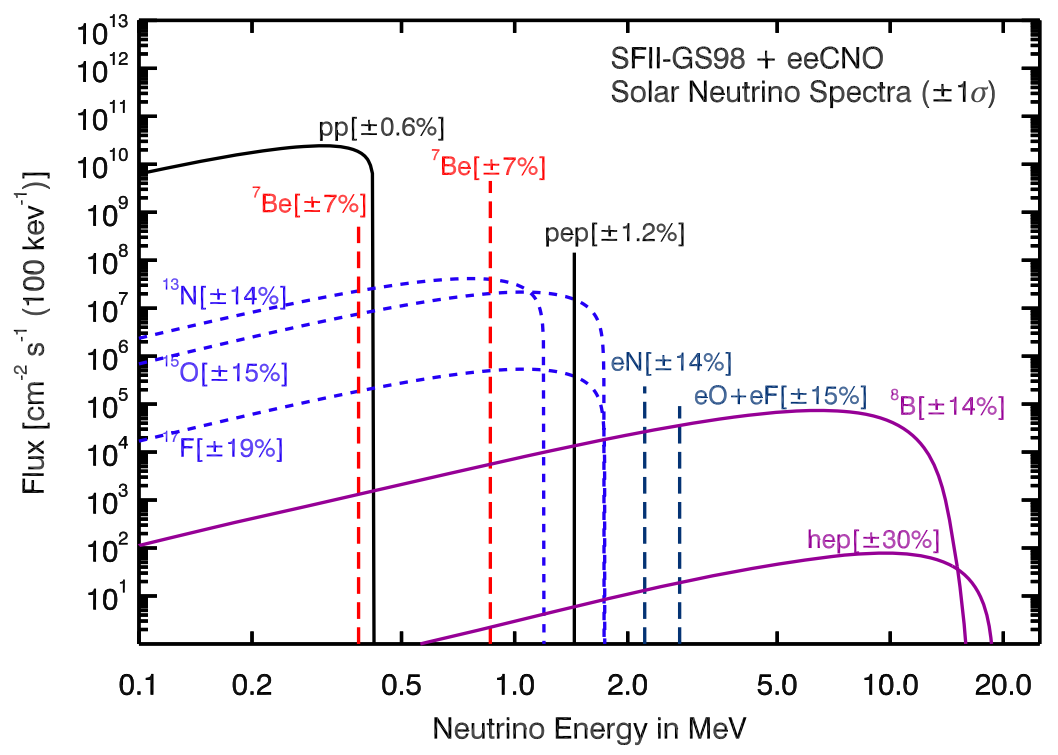
\includegraphics[width=\linewidth]{figures/neutrino-fluxes.png}
    \caption{Energy spectra of solar neutrino fluxes of different reaction processes. Plot taken from \cite{SunNuFluxes}.}
    \label{fig:neutrino-fluxes}
\end{wrapfigure}
As reviewed in \cite{neutrinosPDG}, from which the following discussion is elaborated unless otherwise specified, electron neutrinos are produced in the Sun in thermonuclear reactions that generate solar energy, namely \ac{pp} chains and \ac{CNO} cycles. Based on the \ac{SSM}, the total neutrino flux at Earth can be estimated from the solar luminosity ($L_{\odot} \approx 3.828 \times 10^{26}$~W), dividing it by the net energy released per complete \ac{pp} chain and accounting for the spherical propagation of the neutrinos across the Earth--Sun distance ($1$~AU). In the \ac{pp} chains, which include several neutrino-producing reactions, four protons fuse into a ${}^4$He nucleus, $4p \to {}^4\text{He} + 2e^+ + 2\nu_e$, releasing $Q = 4M({}^1\text{H}) - M({}^4\text{He}) \sim 26.73$~MeV per chain; using atomic masses automatically includes the annihilation of the two positrons with electrons of the plasma. Only a small fraction of this energy, on average $\langle E_{2\nu}\rangle \simeq 0.59$~MeV, is carried away by the two neutrinos, while the rest heats the Sun and is eventually radiated as photons.

In the \ac{CNO} cycles, neutrinos are mainly produced via the decays of ${}^{13}\text{N}$, ${}^{15}\text{O}$ and ${}^{17}\text{F}$. Additionally, electron capture on ${}^{13}\text{N}$, ${}^{15}\text{O}$ and ${}^{17}\text{F}$ produces monoenergetic line spectra of neutrinos, generally referred to as \textit{ecCNO} neutrinos. Compared to the \ac{pp} chains, \ac{CNO} neutrinos carry away a higher fraction of the reaction energy, with average neutrino energies typically ranging between $0.7$~MeV and $1.2$~MeV. However, the flux of \ac{CNO} neutrinos is roughly two orders of magnitude lower than the \ac{pp} one, the \ac{CNO} cycles accounting for less than $1\%$ of the solar energy production, so that they can be neglected in the flux estimate.

Both \ac{pp} reactions and \ac{CNO} ones produce only $\nu_e$: in the absence of oscillations, state-of-the-art calculations predict a \ac{pp} neutrino flux at Earth of approximately $\Phi_\text{pp}(\nu_e) \approx 6 \times 10^{10}~\text{cm}^{-2}\,\text{s}^{-1}$, while the expected fluxes of the individual components are shown in Figure~\ref{fig:neutrino-fluxes}.

\paragraph{The Homestake mine experiment}
Solar neutrinos have been detected since the late 1960s. The first solar neutrino experiment, led by Raymond Davis, was performed underground in the Homestake gold mine in South Dakota, in order to prevent contamination from cosmic-ray induced reactions, which produce ${}^{37}\text{Ar}$ through (p,\,n) processes. It employed liquid tetrachloroethylene (C$_2$Cl$_4$) as the target, exploiting the \ac{CC} interaction $\nu_e + {}^{37}\text{Cl} \longrightarrow e^- + {}^{37}\text{Ar}$, whose threshold of $814$~keV makes it mainly sensitive to ${}^{7}$Be and ${}^{8}$B neutrinos. The produced ${}^{37}\text{Ar}$, with a half-life of $34.8$~days, was chemically extracted every few months and introduced into a low-background proportional chamber, where the Auger electrons emitted in its electron capture were counted to determine the neutrino-${}^{37}\text{Cl}$ reaction rate. The measured rate was less than one third of the expected one, giving rise to the so-called \textit{solar neutrino problem}: the final result was $2.56 \pm 0.16 \pm 0.16 \text{ SNU}$\footnote{SNU (solar neutrino unit) is a unit of event rate defined as $1 \text{ SNU} = 10^{-36}\text{ captures per second per target atom}$. The measured quantity is a capture rate, $R = \sum_i \Phi_i \sigma_i$, summed over the solar neutrino components $i$; converting it into a flux requires assuming the shape of the spectrum.}~\cite{HomestakeResults}, to be compared with the \ac{SSM} prediction of $8.46^{+0.87}_{-0.88} \text{ SNU}$~\cite{SSMReference}.

\paragraph{Gallium-based experiments}
Later, at the turn of the 1990s, two radiochemical experiments were launched: SAGE at the Baksan Neutrino Observatory and GALLEX (later followed by the Gallium Neutrino Observatory, GNO) at the Laboratori Nazionali del Gran Sasso (LNGS). Both exploited the gallium \ac{CC} interaction $\nu_e + {}^{71}\text{Ga} \longrightarrow e^- + {}^{71}\text{Ge}$, whose low threshold of $233$~keV makes it sensitive mainly to \ac{pp} neutrinos, with secondary contributions from ${}^{7}\text{Be}$ ones, i.e. to the lower-energy components of the spectrum of Figure~\ref{fig:neutrino-fluxes}. Following an approach analogous to Homestake, the produced ${}^{71}\text{Ge}$ nuclei, which decay via electron capture with a half-life of $11.4$~days, were chemically extracted to measure the capture rate. SAGE reported $65.4^{+3.1+2.6}_{-3.0-2.8}$ SNU and GALLEX/GNO $69.3 \pm 4.1 \pm 3.6$ SNU, both in sharp contrast with the \ac{SSM} prediction of $127.9^{+8.1}_{-8.2}$ SNU for the same energy range, reinforcing the solar neutrino deficit puzzle.

\paragraph{The Kamiokande experiment}
Starting from the late 1980s, the Kamiokande and Super-Kamiokande water Cherenkov detectors, located in the Kamioka mine in Japan, pioneered real-time measurements of solar neutrino fluxes via \ac{ES} on electrons, written in Eq.~\ref{eq:CC-NCwater} and displayed in Figure~\ref{fig:feynman-CCandNCint}. Kamiokande employed $3000$~t of water, while its successor Super-Kamiokande, running since 1996, contains $50$~kt of ultrapure water.
\begin{equation}
    \label{eq:CC-NCwater}
    \nu_\ell + e^- \longrightarrow \nu_\ell + e^-
\end{equation}
\begin{figure}[H]
    \centering
    \resizebox{0.7\textwidth}{!}{
        % --- Diagramma 1: Corrente Carica (CC) ---
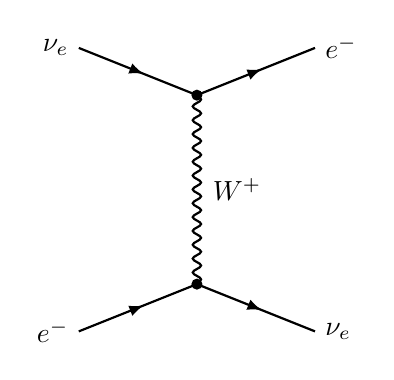
\begin{tikzpicture}[
    thick,
    fermion/.style={draw=black, postaction={decorate},
        decoration={markings, mark=at position 0.55 with {\arrow{latex}}}},
    boson/.style={draw=black, decorate,
        decoration={snake, amplitude=1.5pt, segment length=5pt}},
    dot/.style={circle, fill=black, minimum size=4pt, inner sep=0pt}
]
    \coordinate (V1) at (0, 1.2);
    \coordinate (V2) at (0, -1.2);
    
    \draw[fermion] (-1.5, 1.8) node[left] {$\nu_e$} -- (V1);
    \draw[fermion] (V1) -- (1.5, 1.8) node[right] {$e^-$};
    \draw[fermion] (-1.5, -1.8) node[left] {$e^-$} -- (V2);
    \draw[fermion] (V2) -- (1.5, -1.8) node[right] {$\nu_e$};
    
    \draw[boson] (V1) -- node[right, xshift=2pt] {$W^+$} (V2);
    
    \node[dot] at (V1) {};
    \node[dot] at (V2) {};
\end{tikzpicture}
\hspace{2.5 cm}
% --- Diagramma 2: Corrente Neutra (NC) ---
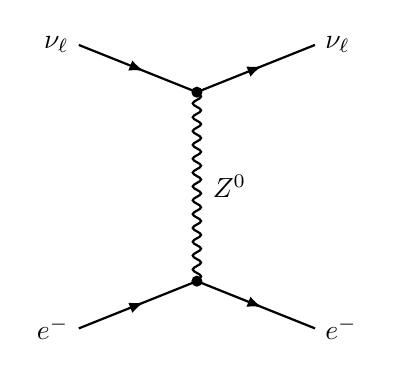
\begin{tikzpicture}[
    thick,
    fermion/.style={draw=black, postaction={decorate},
        decoration={markings, mark=at position 0.55 with {\arrow{latex}}}},
    boson/.style={draw=black, decorate,
        decoration={snake, amplitude=1.5pt, segment length=5pt}},
    dot/.style={circle, fill=black, minimum size=4pt, inner sep=0pt}
]
    \coordinate (V3) at (0, 1.2);
    \coordinate (V4) at (0, -1.2);
    
    \draw[fermion] (-1.5, 1.8) node[left] {$\nu_\ell$} -- (V3);
    \draw[fermion] (V3) -- (1.5, 1.8) node[right] {$\nu_\ell$};
    \draw[fermion] (-1.5, -1.8) node[left] {$e^-$} -- (V4);
    \draw[fermion] (V4) -- (1.5, -1.8) node[right] {$e^-$};
    
    \draw[boson] (V3) -- node[right, xshift=2pt] {$Z^0$} (V4);
    
    \node[dot] at (V3) {};
    \node[dot] at (V4) {};
\end{tikzpicture}
    }
    \caption{Feynman diagrams of neutrino-electron scatterings. On the left, the \ac{CC} interaction mediated by a $W^+$ boson; on the right, the \ac{NC} 
    interaction mediated by the $Z^0$ boson. The subscript $\ell$ denotes a generic lepton flavour ($\ell = e, \mu, \tau$).}
    \label{fig:feynman-CCandNCint}
\end{figure}
This signal is an indistinguishable mixture of \ac{CC} and \ac{NC} events, dominated by $\nu_e$ thanks to its larger cross-section: being the only flavour that can also interact via the \ac{CC}, $\nu_e$ has a cross-section approximately six times larger than that of $\nu_\mu$ or $\nu_\tau$, so that the detector cannot cleanly measure the total, flavour-independent neutrino flux. Due to energy thresholds of $6.5$~MeV in Kamiokande and $3.5$~MeV in Super-Kamiokande, these experiments are sensitive mainly to ${}^8\text{B}$ neutrinos: Super-Kamiokande measured a flux of $(2.345 \pm 0.014 \pm 0.036) \times 10^{6} \text{ cm}^{-2}\text{s}^{-1}$~\cite{latestSUPERK}. This reveals a severe deficit compared to the theoretical \ac{SSM} prediction for ${}^8\text{B}$ neutrinos of $(5.46 \pm 0.66) \times 10^{6} \text{ cm}^{-2}\text{s}^{-1}$.

\paragraph{Solution to the solar neutrino problem: the SNO experiment}
Finally, the Sudbury Neutrino Observatory (SNO), located in the Creighton Mine near Sudbury (Ontario, Canada) and operated between the late 1990s and the early 2000s, provided the model-independent proof that solar $\nu_e$ change flavour, using $1000$~t of heavy water ($\text{D}_2\text{O}$) contained in a spherical acrylic vessel surrounded by a light-water ($\text{H}_2\text{O}$) shield. Deuterium allowed SNO to observe ${}^8\text{B}$ neutrinos not only through the \ac{ES} channel of Eq.~\ref{eq:CC-NCwater}, as Kamiokande, but also to measure separately the \ac{CC} interaction, sensitive only to $\nu_e$, and the \ac{NC} interaction, which breaks the deuteron apart and is sensitive to all active flavours with equal cross-sections. Both interactions are written in Eq.~\ref{eq:deuteron-interactions} and shown in Figure~\ref{fig:feynman-deuteron}.
\begin{equation}
    \label{eq:deuteron-interactions}
    \begin{aligned}
        \nu_e + d &\longrightarrow e^- + p + p \quad (\text{\ac{CC}})\\
        \nu_\ell + d &\longrightarrow \nu_\ell + p + n \quad (\text{\ac{NC}})
    \end{aligned}
\end{equation}
\begin{figure}[H]
    \centering
    \resizebox{0.7\textwidth}{!}{
        % --- Diagramma 1: Corrente Carica (CC) per SNO ---
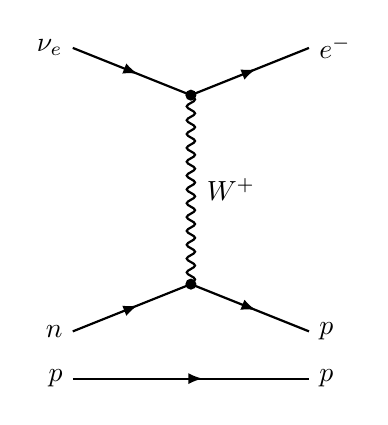
\begin{tikzpicture}[
    thick,
    fermion/.style={draw=black, postaction={decorate},
        decoration={markings, mark=at position 0.55 with {\arrow{latex}}}},
    boson/.style={draw=black, decorate,
        decoration={snake, amplitude=1.5pt, segment length=5pt}},
    dot/.style={circle, fill=black, minimum size=4pt, inner sep=0pt}
]
    \coordinate (V1) at (0, 1.2);
    \coordinate (V2) at (0, -1.2);
    
    % Linea superiore: neutrino -> elettrone
    \draw[fermion] (-1.5, 1.8) node[left] {$\nu_e$} -- (V1);
    \draw[fermion] (V1) -- (1.5, 1.8) node[right] {$e^-$};
    
    % Linee inferiori: neutrone che diventa protone, e protone spettatore
    \draw[fermion] (-1.5, -1.8) node[left] {$n$} -- (V2);
    \draw[fermion] (V2) -- (1.5, -1.8) node[right] {$p$};
    \draw[fermion] (-1.5, -2.4) node[left] {$p$} -- (1.5, -2.4) node[right] {$p$};
    
    % Bosone scambiato W+
    \draw[boson] (V1) -- node[right, xshift=2pt] {$W^+$} (V2);
    
    \node[dot] at (V1) {};
    \node[dot] at (V2) {};
\end{tikzpicture}
\hspace{2.5 cm}
% --- Diagramma 2: Corrente Neutra (NC) per SNO ---
\begin{tikzpicture}[
    thick,
    fermion/.style={draw=black, postaction={decorate},
        decoration={markings, mark=at position 0.55 with {\arrow{latex}}}},
    boson/.style={draw=black, decorate,
        decoration={snake, amplitude=1.5pt, segment length=5pt}},
    dot/.style={circle, fill=black, minimum size=4pt, inner sep=0pt}
]
    \coordinate (V3) at (0, 1.2);
    \coordinate (V4) at (0, -1.2);
    
    % Linea superiore: neutrino -> elettrone
    \draw[fermion] (-1.5, 1.8) node[left] {$\nu_\ell$} -- (V3);
    \draw[fermion] (V1) -- (1.5, 1.8) node[right] {$\nu_\ell$};
    
    % Linee inferiori: neutrone che diventa protone, e protone spettatore
    \draw[fermion] (-1.5, -1.8) node[left] {$n$} -- (V4);
    \draw[fermion] (V2) -- (1.5, -1.8) node[right] {$n$};
    \draw[fermion] (-1.5, -2.4) node[left] {$p$} -- (1.5, -2.4) node[right] {$p$};

    % Bosone scambiato Z0
    \draw[boson] (V3) -- node[right, xshift=2pt] {$Z^0$} (V4);
    
    \node[dot] at (V3) {};
    \node[dot] at (V4) {};
\end{tikzpicture}
    }
    \caption{Feynman diagrams of neutrino-deuteron scatterings. On the left, the \ac{CC} interaction mediated by a $W^+$ boson; on the right, the \ac{NC} 
    interaction mediated by the $Z^0$ boson. The subscript $\ell$ denotes a generic lepton flavour ($\ell = e, \mu, \tau$).}
    \label{fig:feynman-deuteron}
\end{figure}
The ${}^{8}\text{B}$ neutrino fluxes measured in the three channels are reported in Eq.~\ref{eq:SNOresults}~\cite{SNO2002-results}:
\begin{equation}
    \label{eq:SNOresults}
    \begin{aligned}
        \Phi_\text{SNO}^\text{CC}(\nu_e) &= (1.76 \pm 0.05 \pm 0.09) \times 10^{6}~\text{cm}^{-2}\,\text{s}^{-1} \\
        \Phi_\text{SNO}^\text{ES}(\nu_\ell) &= (2.39 \pm 0.24 \pm 0.12) \times 10^{6}~\text{cm}^{-2}\,\text{s}^{-1} \\
        \Phi_\text{SNO}^\text{NC}(\nu_\ell) &= (5.09 \pm 0.44 \pm 0.46) \times 10^{6}~\text{cm}^{-2}\,\text{s}^{-1}
    \end{aligned}
\end{equation} 
The total active flux measured by the \ac{NC} channel is in agreement with the \ac{SSM} prediction, both with the historical ones of that era and with the updated value of $(5.46 \pm 0.66) \times 10^{6} \text{ cm}^{-2}\text{s}^{-1}$ quoted above, while the \ac{CC} channel, sensitive only to $\nu_e$, measured a much lower flux. The ratio $\Phi^\text{CC}_\text{SNO}/\Phi^\text{NC}_\text{SNO}  \simeq 0.35$ shows that about two thirds of the $\nu_e$ produced in the solar core reach the Earth as $\nu_\mu$ or $\nu_\tau$. The first conclusive evidence for neutrino oscillations had been obtained in 1998 by Super-Kamiokande with atmospheric neutrinos, through the up-down asymmetry of the $\nu_\mu$ flux~\cite{SuperK1998}.

The different deficit ratios observed by radiochemical experiments (Homestake, SAGE, GALLEX/GNO) and water Cherenkov detectors (Super-Kamiokande, SNO) arise because each experiment probes a different part of the solar neutrino energy spectrum, over which the $\nu_e$ survival probability varies. In the standard picture, this energy dependence results from the transition between vacuum-dominated oscillations at low energies and matter-enhanced conversion inside the Sun at high energies. The following two sections outline these two regimes, starting from the simpler case of oscillations in vacuum, whose formalism is also the basis for including matter effects.


% ----------------------------------------------------------
% ------------------- VACUUM OCILLATIONS -------------------
% ----------------------------------------------------------

\subsection{Vacuum oscillations}
\label{subsec:VacuumOscillations}

Following the treatment of \cite{Thomson}, flavour oscillations can be understood as a consequence of the fact that the neutrino states produced and detected in weak interactions, the flavour eigenstates, do not coincide with the states of definite mass. The physical states of a free particle, i.e. the mass eigenstates, are the stationary states of the free-particle Hamiltonian, satisfying Eq.~\ref{eq:free-hamiltonian} and following the time evolution of Eq.~\ref{eq:time-evolution}.
\begin{equation}
    \label{eq:free-hamiltonian}
    \hat{H} \psi = i \frac{\partial \psi}{\partial t} = E \psi
\end{equation}
\begin{equation}
    \label{eq:time-evolution}
    \psi(\text{\textbf{x}}, \text{t}) = \varphi (\text{\textbf{x}}) e ^{-i \text{Et}}
\end{equation}
The neutrino mass eigenstates that obey Eqs.~\ref{eq:free-hamiltonian} and~\ref{eq:time-evolution} are labelled $\nu_1$, $\nu_2$ and $\nu_3$, and there is no reason to believe that such states correspond to the neutrino weak eigenstates $\nu_e$, $\nu_\mu$ and $\nu_\tau$, which are identified when the corresponding charged lepton is produced. For charged leptons, instead, flavour and mass eigenstates can be taken to coincide, as discussed at the end of this section.

Consider the lepton SU(2)$_\text{L}$ doublet of a given family $i = 1, 2, 3$. This can be written as
\begin{equation}
    \label{eq:weak-lepton-doublet}
    L_{\text{L}, i} = \begin{pmatrix}
                            \nu'_{\text{L}} \\
                            \ell'_{\text{L}}
                      \end{pmatrix}_i ,
\end{equation}
where the primes denote fields in the basis in which they enter the gauge interactions (\textit{weak basis}), and it is precisely this multiplet that couples to the electroweak gauge bosons in the weak sector of the \ac{SM} Lagrangian written in Eq.~\ref{eq:lepton-interaction}, with an implicit sum over $i$.
\begin{equation}
    \label{eq:lepton-interaction}
    \mathcal{L}_{\text{int}} = - \bar{L}_{\text{L}, i} \gamma^\mu \left( g \frac{\tau^a}{2} W_\mu^a + g' Y B_\mu \right) L_{\text{L}, i}
\end{equation}

However, when the \ac{SSB} happens, the charged leptons acquire mass through their Yukawa couplings to the Higgs field; if neutrinos are massive as well, which requires a neutrino mass term not present in the minimal \ac{SM} (see Section~\ref{subsec:seesaw}), the fields of the weak doublet can be expressed in terms of the mass eigenstates as written in Eq.~\ref{eq:weak-mass-transformation}
\begin{equation}
    \label{eq:weak-mass-transformation}
    \begin{cases}
        \nu'_{\text{L}, i} = \sum_{j} \left(U_{\nu \text{L}}\right)_{ij}\, \nu_{\text{L}, j} \\[1ex]
        \ell'_{\text{L}, i} = \sum_{j} \left(U_{\ell \text{L}}\right)_{ij}\, \ell_{\text{L}, j}
    \end{cases}
\end{equation}
where $\nu_{\text{L}, j}$ and $\ell_{\text{L}, j}$ are the mass eigenstates of neutrinos and charged leptons respectively, and $U_{\nu\text{L}}$ and $U_{\ell\text{L}}$ are the unitary matrices that diagonalise the corresponding mass matrices. Consequently, the charged-current terms undergo the transformation expressed in Eq.~\ref{eq:current-masseigen}
\begin{equation}
    \label{eq:current-masseigen}
    \sum_i \bar{\ell}'_{\text{L}, i}\, \gamma^{\mu}\, \nu'_{\text{L}, i}
    = \sum_{j,k} \bar{\ell}_{\text{L}, j}\, \gamma^{\mu}
      \big(\underbrace{U_{\ell \text{L}}^\dagger U_{\nu \text{L}}}_{U_{\text{PMNS}}}\big)_{jk}\,
      \nu_{\text{L}, k}
\end{equation}
where a new matrix can be highlighted: the Pontecorvo-Maki-Nakagawa-Sakata ($U_\text{PMNS}$) mixing matrix\footnote{Such rotation matrix is the leptonic equivalent of the Cabibbo-Kobayashi-Maskawa ($V_\text{CKM}$) matrix for the quark sector of the \ac{SM}, with the proper adaptations to be considered.}. 
Named in honour of the physicists who first formulated its theoretical framework~\cite{Pontecorvo1957, Pontecorvo1967, Maki1962}, 
this matrix establishes a link between the weak (flavour) eigenstates, i.e. $\nu_e$, $\nu_\mu$ and $\nu_\tau$, 
and the stationary (mass) eigenstates, i.e. $\nu_1$, $\nu_2$ and $\nu_3$,
as detailed in Eq.~\ref{eq:Upmns}. 
\begin{equation}
    \label{eq:Upmns}
    \begin{pmatrix}
    \nu_e \\
    \nu_\mu \\
    \nu_\tau
    \end{pmatrix}
    =
    \begin{pmatrix}
    U_{e1} & U_{e2} & U_{e3} \\
    U_{\mu1} & U_{\mu2} & U_{\mu3} \\
    U_{\tau1} & U_{\tau2} & U_{\tau3}
    \end{pmatrix}
    \begin{pmatrix}
    \nu_1 \\
    \nu_2 \\
    \nu_3
\end{pmatrix}
\end{equation}

It should be stressed that $U_\text{PMNS}$ is physical only because $U_{\ell\text{L}}$ and $U_{\nu\text{L}}$ are fixed independently by two different mass matrices. In the minimal \ac{SM} there is no \ac{RH} neutrino, hence no neutrino mass term: nothing in the Lagrangian fixes the neutrino basis, so $U_{\nu\text{L}}$ is arbitrary and can be chosen equal to $U_{\ell\text{L}}$. In that case $U_\text{PMNS} = \mathbb{1}$, the charged current is diagonal and the family lepton numbers $L_e$, $L_\mu$ and $L_\tau$ are separately conserved. Mixing is observable only if the neutrino mass matrix is not aligned with the charged-lepton one and the neutrino masses are not degenerate, since for degenerate masses any rotation within the degenerate subspace could be used to remove it. The observation of flavour oscillations therefore implies that at least two neutrinos are massive, which requires physics beyond the minimal \ac{SM}.

This matrix is a $3 \times 3$ unitary matrix that parametrises a rotation (a mixing) through some parameters. A general $3 \times 3$ matrix can be written in terms of 9 complex numbers, i.e., 18 parameters; however, the unitarity property of $U_{\text{PMNS}}$, which means $U U^\dagger = \mathbb{1}$, introduces nine constraints, leaving only nine independent parameters to fully describe the mixing. Among these nine parameters, three of them are angles, $\theta_{12}$, $\theta_{13}$, $\theta_{23}$, while the remaining six are complex phases of the form $e^{i \varphi}$, since $U_{\text{PMNS}}$ is not a real matrix. Specifically, $\theta_{12}$ is the angle of rotation about the 3-axis, $\theta_{13}$ is the angle of rotation about the new 2-axis and $\theta_{23}$ is a rotation about the remaining 1-axis.

Not all of the six phases are physical. The charged-current interaction, together with the Dirac mass terms, is invariant under the rephasing of the charged-lepton fields $\ell_\alpha$ ($\alpha = e, \mu, \tau$) and of the neutrino mass-eigenstate fields $\nu_k$ ($k = 1, 2, 3$),
\begin{equation}
    \ell_\alpha \longrightarrow e^{i\theta_\alpha}\,\ell_\alpha \qquad \text{and} \qquad \nu_k \longrightarrow e^{i\theta_k}\,\nu_k ,
\end{equation}
provided that the mixing matrix transforms as
\begin{equation}
    U_{\alpha k} \longrightarrow e^{i(\theta_\alpha - \theta_k)}\, U_{\alpha k}.
\end{equation}
This gives six free phases, three $\theta_\alpha$ and three $\theta_k$, but only their differences enter. In particular, a common shift $\theta_\alpha = \theta_k = \theta$ leaves every $U_{\alpha k}$ unchanged, so only $6 - 1 = 5$ phases can actually be used to remove phases from $U_\text{PMNS}$. Five of the six phases are therefore unphysical.

The number of physical phases that remain depends on the nature of neutrinos. If neutrinos are Dirac particles (meaning that they are distinct from their antiparticles), $U_\text{PMNS}$ is described by four physical parameters: the three mixing angles $\theta_{12}$, $\theta_{13}$, $\theta_{23}$ and a single irreducible phase $\delta$, which is responsible for \ac{CP} violation in the lepton sector.

If instead neutrinos are Majorana particles (meaning that they are their own antiparticles, a possibility discussed in Section~\ref{subsec:seesaw}), the Majorana mass term $\nu_k^T C \nu_k$ is not invariant under the rephasing of $\nu_k$. Only the three phases $\theta_\alpha$ can then be used, so two additional physical phases survive, known as Majorana phases $\alpha_{21}$ and $\alpha_{31}$, bringing the total number of physical parameters to six. They enter as a diagonal matrix multiplying $U_\text{PMNS}$ on the right,
\begin{equation}
    \label{eq:Upmns-majorana}
    U_\text{PMNS}^\text{Maj} = U_\text{PMNS}\;\text{diag}\left(1,\, e^{i\alpha_{21}/2},\, e^{i\alpha_{31}/2}\right),
\end{equation}
and cancel in the neutrino oscillation probabilities, which therefore cannot distinguish Dirac from Majorana neutrinos. The Majorana phases are accessible only through lepton-number-violating processes such as neutrinoless double $\beta$-decay (Section~\ref{sec:0nubetabeta}).

Finally, the full neutrino mixing matrix can be written as reported in Eq.~\ref{eq:Upmns-total}
\begin{equation}
    \label{eq:Upmns-total}
    U_{\text{PMNS}} = 
    \begin{pmatrix}
    U_{e1} & U_{e2} & U_{e3} \\
    U_{\mu 1} & U_{\mu 2} & U_{\mu 3} \\
    U_{\tau 1} & U_{\tau 2} & U_{\tau 3}
    \end{pmatrix}
    =
    \begin{pmatrix}
    c_{12}c_{13} & s_{12}c_{13} & s_{13}e^{-i\delta} \\[1ex]
    -s_{12}c_{23} - c_{12}s_{23}s_{13}e^{i\delta} & c_{12}c_{23} - s_{12}s_{23}s_{13}e^{i\delta} & s_{23}c_{13} \\[1ex]
    s_{12}s_{23} - c_{12}c_{23}s_{13}e^{i\delta} & -c_{12}s_{23} - s_{12}c_{23}s_{13}e^{i\delta} & c_{23}c_{13}
    \end{pmatrix}
\end{equation}

or, equivalently, factorised in the product of the three matrices detailed in Eq.~\ref{eq:Upmns-factorised}
\begin{equation}
    \label{eq:Upmns-factorised}
    U_{\text{PMNS}} = 
    \begin{pmatrix}
    1 & 0 & 0 \\
    0 & c_{23} & s_{23} \\
    0 & -s_{23} & c_{23}
    \end{pmatrix}
    \begin{pmatrix}
    c_{13} & 0 & s_{13}e^{-i\delta} \\
    0 & 1 & 0 \\
    -s_{13}e^{i\delta} & 0 & c_{13}
    \end{pmatrix}
    \begin{pmatrix}
    c_{12} & s_{12} & 0 \\
    -s_{12} & c_{12} & 0 \\
    0 & 0 & 1
    \end{pmatrix}
\end{equation}

where $s_{ij} = \sin(\theta_{ij})$ and $c_{ij} = \cos(\theta_{ij})$.

Since $U_\text{PMNS} = U_{\ell\text{L}}^\dagger U_{\nu\text{L}}$, only the relative rotation between the two bases is physical, and the mixing could in principle be attributed to the charged leptons as well. The convention of assigning it to neutrinos follows from how leptons are observed: charged leptons are identified through their masses, so that their flavour and mass eigenstates coincide by definition, while neutrinos are never detected directly and their flavour is defined by the charged lepton produced in the \ac{CC} interaction. The neutrino flavour states are therefore coherent superpositions of the mass eigenstates, through the mixing matrix $U_\text{PMNS}$.

A detailed analysis of three-flavour neutrino oscillations is given below.

\paragraph{Three-flavour neutrino oscillation}
\label{par:ThreeFlavoursOscillation}
This paragraph provides the mathematical derivation of the neutrino survival and oscillation probabilities within a three-flavour oscillation framework, elaborated from \cite{Brugnera}.

Consider an electron neutrino produced at $t=0$. It can be written as 
\begin{equation*}
    | \psi(0) \rangle = | \nu_e \rangle = U_{e1}^* | \nu_1 \rangle + U_{e2}^* | \nu_2 \rangle + U_{e3}^* | \nu_3 \rangle
\end{equation*}
Such state evolves in time, and in space as well, according to the time dependence of the mass eigenstates; thus, after travelling for a time $t$ and a distance $\mathbf{x}$, we can write
\begin{equation}
    \label{eq:psi-time-evolution}
    | \psi(\mathbf{x}, t) \rangle = U_{e1}^* | \nu_1 \rangle e^{-i\phi_1} + U_{e2}^* | \nu_2 \rangle e^{-i\phi_2} + U_{e3}^* | \nu_3 \rangle e^{-i\phi_3}.
\end{equation}
In Eq.~\ref{eq:psi-time-evolution}, $\phi_1$, $\phi_2$ and $\phi_3$ are the quantum mechanical phases accumulated by each mass eigenstate.
For a generic state $i$, with $i = 1, 2, 3$, the Lorentz-invariant phase is given by $\phi_i = p^\mu_i x_\mu = E_i t - \mathbf{p}_i \cdot \mathbf{x}$, where $p^\mu_i = (E_i, \mathbf{p}_i)$
is the four-momentum of the $i$-th mass eigenstate and $x_\mu = (t, \mathbf{x})$ is the macroscopic spacetime coordinate of the state.
It is crucial to note that, while the spacetime coordinate is common to the entire superposition, 
the energy $E_i$ and the three-momentum $\mathbf{p}_i$ of each component fundamentally depend on its specific mass $m_i$ through the relativistic 
relation $E_i^2 = |\mathbf{p}_i|^2 + m_i^2$.

We can then express $| \nu_1 \rangle$, $| \nu_2 \rangle$ and $| \nu_3 \rangle$ in terms of $| \nu_e \rangle$, $| \nu_\mu \rangle$ and 
$| \nu_\tau \rangle$, obtaining
\begin{equation*}
    \begin{aligned}
        | \psi(\mathbf{x}, t) \rangle = \;& U_{e1}^* (U_{e1} | \nu_e \rangle + U_{\mu 1} | \nu_\mu \rangle + U_{\tau 1} | \nu_\tau \rangle) e^{-i\phi_1} \\
        &+ U_{e2}^* (U_{e2} | \nu_e \rangle + U_{\mu 2} | \nu_\mu \rangle + U_{\tau 2} | \nu_\tau \rangle) e^{-i\phi_2} \\
        &+ U_{e3}^* (U_{e3} | \nu_e \rangle + U_{\mu 3} | \nu_\mu \rangle + U_{\tau 3} | \nu_\tau \rangle) e^{-i\phi_3}.
    \end{aligned}
\end{equation*}
Grouping together all the terms referring to the same flavour eigenstate, we get
\begin{equation}
    \label{eq:evolved-state}
    \begin{aligned}
        | \psi(\mathbf{x}, t) \rangle &= \underbrace{(U_{e1}^* U_{e1} e^{-i\phi_1} + U_{e2}^* U_{e2} e^{-i\phi_2} + U_{e3}^* U_{e3} e^{-i\phi_3})}_{c_e} | \nu_e \rangle \\
        &+ \underbrace{(U_{e1}^* U_{\mu 1} e^{-i\phi_1} + U_{e2}^* U_{\mu 2} e^{-i\phi_2} + U_{e3}^* U_{\mu 3} e^{-i\phi_3})}_{c_\mu} | \nu_\mu \rangle \\
        &+ \underbrace{(U_{e1}^* U_{\tau 1} e^{-i\phi_1} + U_{e2}^* U_{\tau 2} e^{-i\phi_2} + U_{e3}^* U_{\tau 3} e^{-i\phi_3})}_{c_\tau} | \nu_\tau \rangle
    \end{aligned}
\end{equation}
Consequently, to compute the probability that the initial electron neutrino $| \psi(0) \rangle$ oscillates into a muon or a tau neutrino
after a time $t$ and a distance $\mathbf{x}$, we just need to project the state at $(\mathbf{x}, t)$ onto the specific flavour eigenstate. 
As an example, the oscillation probability $P(\nu_{e} \rightarrow \nu_\mu)$ yields
\begin{equation}
    \label{eq:oscillation-prob}
    \begin{aligned}
        P(\nu_{e} \rightarrow \nu_\mu) &= | \langle \nu_\mu | \psi(\mathbf{x}, t) \rangle|^2 = c_\mu^* c_\mu = |c_\mu|^2 = \\
                    &= \left|U_{e1}^* U_{\mu 1} e^{-i\phi_1} + U_{e2}^* U_{\mu 2} e^{-i\phi_2} + U_{e3}^* U_{\mu 3} e^{-i\phi_3}\right|^2.
    \end{aligned}
\end{equation}
Exploiting the complex-number identity $|z_1 +z_2 +z_3|^2 = |z_1|^2 + |z_2|^2 + |z_3|^2 + 2\,\Re\{z_1z_2^* + z_1z_3^* + z_2z_3^*\}$, 
Eq.~\ref{eq:oscillation-prob} can be rewritten as shown in Eq.~\ref{eq:oscillation-prob-revisited}
\begin{equation}
    \label{eq:oscillation-prob-revisited}
    \begin{aligned}
        P(\nu_e \to \nu_\mu) &= |U_{e1}^* U_{\mu 1}|^2 + |U_{e2}^* U_{\mu 2}|^2 + |U_{e3}^* U_{\mu 3}|^2 + 2\,\Re \left\{ U_{e1}^* U_{\mu 1} U_{e2} U_{\mu 2}^* e^{-i(\phi_1 - \phi_2)} \right\} \\
        &\quad + 2\,\Re \left\{ U_{e1}^* U_{\mu 1} U_{e3} U_{\mu 3}^* e^{-i(\phi_1 - \phi_3)} \right\} + 2\,\Re \left\{ U_{e2}^* U_{\mu 2} U_{e3} U_{\mu 3}^* e^{-i(\phi_2 - \phi_3)} \right\}.
    \end{aligned}
\end{equation}
Then we can use complex-number properties together with the unitarity of the PMNS matrix. 
Specifically, the orthogonality condition between the electron and muon flavours dictates that
\begin{equation}
    \label{eq:unitarity-condition}
    U_{e1}^* U_{\mu 1} + U_{e2}^* U_{\mu 2} + U_{e3}^* U_{\mu 3} = 0 .
\end{equation}

By taking the modulus squared of Eq.~\ref{eq:unitarity-condition}, we obtain the expansion shown below:
\begin{equation}
    \label{eq:unitarity-squared}
    \begin{aligned}
        &|U_{e1}^* U_{\mu 1}|^2 + |U_{e2}^* U_{\mu 2}|^2 + |U_{e3}^* U_{\mu 3}|^2 \\
        &+ 2\,\Re \left\{ U_{e1}^* U_{\mu 1} U_{e2} U_{\mu 2}^* + U_{e1}^* U_{\mu 1} U_{e3} U_{\mu 3}^* + U_{e2}^* U_{\mu 2} U_{e3} U_{\mu 3}^* \right\} = 0
    \end{aligned}
\end{equation}

Isolating the sum of the squared moduli in Eq.~\ref{eq:unitarity-squared} and substituting it into the first three terms of Eq.~\ref{eq:oscillation-prob-revisited} yields Eq.~\ref{eq:oscillation-prob-final}.
\begin{equation}
    \label{eq:oscillation-prob-final}
    \begin{aligned}
        P(\nu_e \to \nu_\mu) = &2\,\Re \left\{ U_{e1}^* U_{\mu 1} U_{e2} U_{\mu 2}^* \left[ e^{-i(\phi_1 - \phi_2)} - 1 \right] \right\} \\
        \quad + &2\,\Re \left\{ U_{e1}^* U_{\mu 1} U_{e3} U_{\mu 3}^* \left[ e^{-i(\phi_1 - \phi_3)} - 1 \right] \right\} \\
        \quad + &2\,\Re \left\{ U_{e2}^* U_{\mu 2} U_{e3} U_{\mu 3}^* \left[ e^{-i(\phi_2 - \phi_3)} - 1 \right] \right\}
    \end{aligned}
\end{equation}
Similarly, the electron neutrino survival probability, i.e. $P(\nu_e \to \nu_e)$, is obtained; in this case, however, 
each element of the PMNS matrix is paired with its own complex conjugate (see Eq.~\ref{eq:evolved-state}).
Therefore, we can write
\begin{equation*}
    \begin{aligned}
    P(\nu_e \to \nu_e) = 1 &+ 2 |U_{e1}|^2|U_{e2}|^2 \,\Re\{e^{i(\phi_2-\phi_1)}-1\}\\
                           &+ 2 |U_{e1}|^2|U_{e3}|^2 \,\Re\{e^{i(\phi_3-\phi_1)}-1\}\\
                           &+ 2 |U_{e2}|^2|U_{e3}|^2 \,\Re\{e^{i(\phi_3-\phi_2)}-1\}
    \end{aligned}
\end{equation*}
Furthermore, the mass dependence of the oscillation probabilities can be highlighted through the trigonometric identity of Eq.~\ref{eq:sinDeltaij}
\begin{equation}
    \label{eq:sinDeltaij}
    \Re\{e^{i(\phi_j-\phi_i)}-1\} = \cos(\phi_j-\phi_i) - 1 = -2 \sin^2\left(\frac{\phi_j-\phi_i}{2}\right) = -2 \sin^2(\Delta \phi_{ji})
\end{equation}
The argument of the sine function crucially depends on the phase difference between the mass eigenstates $j$ and $i$. 
Recalling the definition of the Lorentz-invariant phase introduced earlier, and considering a one-dimensional propagation along the baseline 
$L$ (so that $\mathbf{p}_i \cdot \mathbf{x} = p_i L$), this difference is explicitly written as:
\begin{equation}
    \label{eq:phase-diff-general}
    \Delta\phi_{ji} \equiv \frac{\phi_j - \phi_i}{2} = \frac{(E_j - E_i)t - (p_j - p_i)L}{2}
\end{equation}

To express this phase difference in terms of measurable quantities (the baseline $L$ and the neutrino energy $E_\nu$), the standard plane-wave treatment requires some kinematic assumptions. First, one can assume that the different mass eigenstates are produced with the same momentum, $p_i = p_j = p$. Under this assumption, the second term in Eq.~\ref{eq:phase-diff-general} vanishes.

Second, exploiting the relativistic relation $E_i^2 = |\mathbf{p}_i|^2 + m_i^2$ previously mentioned, and since neutrinos are ultra-relativistic 
($m_i \ll p$), we can perform a Taylor expansion:
\begin{equation}
    \label{eq:energy-taylor}
    E_i = \sqrt{p^2 + m_i^2} = p\sqrt{1 + \frac{m_i^2}{p^2}} \approx p \left( 1 + \frac{m_i^2}{2p^2} \right) = p + \frac{m_i^2}{2p}
\end{equation}

Consequently, the energy difference between two mass eigenstates becomes:
\begin{equation}
    \label{eq:energy-diff}
    E_j - E_i \approx \left( p + \frac{m_j^2}{2p} \right) - \left( p + \frac{m_i^2}{2p} \right) = \frac{m_j^2 - m_i^2}{2p}
\end{equation}

Furthermore, in the ultra-relativistic limit the neutrino velocity is $\beta \approx 1$ (in natural units, $c=1$), 
which implies that the time of flight $t$ is well approximated by the distance travelled $L$ ($t \approx L$), 
and the modulus of the neutrino three-momentum $p$ is approximated by its energy $E_\nu$. 
Substituting these into Eq.~\ref{eq:phase-diff-general}, we get:
\begin{equation}
    \label{eq:phase-diff-approx1}
    \Delta\phi_{ji} \equiv \frac{\phi_j - \phi_i}{2} \approx \frac{1}{2}\frac{m_j^2 - m_i^2}{2p}L = \frac{(m_j^2 - m_i^2)L}{4E_\nu}.
\end{equation}
The latter result highlights how oscillation and survival probabilities intrinsically depend on the differences of the squared masses of the neutrino stationary states.

%-----------------------------------------------------------
%------------------- MATTER EFFECT -----------------------
%-----------------------------------------------------------

\subsection{Massive neutrinos in matter}
\label{subsec:nu-in-matter}

In Section~\ref{subsec:oscillation-experiments} we mentioned that the flavour conversion of solar neutrinos can have two different explanations: oscillations in vacuum on their way to the Earth, or flavour conversion within the Sun itself through a matter-mediated process known as the \ac{MSW} effect, that is detailed in what follows on the basis of what reported in \cite{neutrinosPDG}\footnote{The complete quantum mechanical derivation of this effect, starting from the \ac{SM} fermionic currents and phase-space averages, is given in Paragraph~\ref{par:MSW_derivation}.}.

When neutrinos propagate through a dense medium like the solar interior, they interact with the surrounding particles (electrons, protons, and neutrons) via elastic, coherent forward scatterings\footnote{The cross-section of incoherent scatterings is of the order $\sigma \sim \mathcal{O}(10^{-43}\text{cm}^2)$. Therefore, such processes are negligible.}. These coherent interactions macroscopically act as an effective refractive index, which alters the propagation states of the neutrinos.

The fundamental physical asymmetry that drives the \ac{MSW} effect lies in the standard weak interactions. In ordinary matter, all active neutrino flavours ($\nu_e, \nu_\mu, \nu_\tau$) interact with electrons, protons, and neutrons via \ac{NC} interactions mediated by the $Z^0$ boson. Because these interactions are flavour-blind, they induce a common potential for all neutrino flavours. Since neutrino oscillations depend on the \textit{phase differences} between mass eigenstates, this universal \ac{NC} contribution effectively cancels out and does not alter the flavour transition probabilities.

However, ordinary matter is rich in electrons but completely lacks muons and taus. Consequently, only electron neutrinos ($\nu_e$) can undergo \ac{CC} interactions with the electrons in the medium, mediated by the $W^\pm$ bosons. This exclusive interaction provides an additional potential energy strictly for the $\nu_e$ state, known as the Wolfenstein potential:
\begin{equation}
    % \label{eq:V_C_potential}
    V_C = \sqrt{2} G_F n_e
\end{equation}
where $G_F$ is the Fermi coupling constant and $n_e$ is the electron number density of the medium. For antineutrinos, this potential flips its sign ($V_C = -\sqrt{2} G_F n_e$).

This effective potential modifies the Hamiltonian of the system. As a result, both the mass eigenstates and the mixing angles in matter become dependent on the local electron density $n_e$. In the Sun, the effect depends on the neutrino energy. In the two-flavour approximation the mixing angle in matter is
\begin{equation}
    \label{eq:matter-angle}
    \tan 2\theta_m = \frac{\sin 2\theta_{12}}{\cos 2\theta_{12} - A/\Delta m^2_{21}},
    \qquad A = 2\sqrt{2}\, G_F\, n_e\, E,
\end{equation}
and in the solar core matter effects dominate above $E_\text{crit} \simeq \Delta m^2_{21}\cos 2\theta_{12}/(2V_C) \simeq 2$~MeV.

\paragraph{Mathematical derivation of the Mikheyev-Smirnov-Wolfenstein effect}
\label{par:MSW_derivation}
This paragraph provides the full mathematical derivation of the effective potential experienced by electron neutrinos propagating through ordinary matter, starting from the \ac{SM} fermionic currents. It is based on \cite{neutrinosPDG}.

Consider the evolution of a $\nu_e$ in a medium with electron, proton and neutron number densities $n_e$, $n_p$ and $n_n$, respectively. The effective Hamiltonian describing the relevant neutrino interactions at a point $x$ is given in Eq.~\ref{eq:effHamiltonian-matter}
\begin{equation}
    \label{eq:effHamiltonian-matter}
    H_W = \frac{G_F}{\sqrt{2}} \left[ J^{(+)\alpha}(x) J^{(-)}_\alpha(x) + \frac{1}{4} J^{(N)\alpha}(x) J^{(N)}_\alpha(x) \right],
\end{equation}
where the fermionic currents are the following, with $g_A^{(n, p)}$ the axial couplings of neutrons and protons:
\begin{equation}
    \label{eq:fermionic-currents}
    \begin{aligned}
        J^{(+)}_\alpha(x) &= \overline{\nu}_e(x) \gamma_\alpha (1 - \gamma_5) e(x), \\
        J^{(-)}_\alpha(x) &= \overline{e}(x) \gamma_\alpha (1 - \gamma_5) \nu_e(x), \\
        J^{(N)}_\alpha(x) &= \overline{\nu}_e(x) \gamma_\alpha (1 - \gamma_5) \nu_e(x) \\
        &\quad - \overline{e}(x) \left[ \gamma_\alpha(1 - \gamma_5) - 4\sin^2\theta_W \gamma_\alpha \right] e(x) \\
        &\quad + \overline{p}(x) \left[ \gamma_\alpha(1 - g_A^{(p)}\gamma_5) - 4\sin^2\theta_W \gamma_\alpha \right] p(x) \\
        &\quad - \overline{n}(x) \gamma_\alpha (1 - g_A^{(n)}\gamma_5) n(x).
    \end{aligned}
\end{equation}
Firstly, we focus on the \ac{CC} part. The effective \ac{CC} Hamiltonian arising from the interactions with the electrons of the medium is
\begin{equation}
    \label{eq:H_C_e_1}
    \begin{aligned}
        H_C^{(e)} &= \frac{G_F}{\sqrt{2}} \int d^3p_e f(E_e, T) \times \boldsymbol{\Big\langle} e(s, p_e) \mid \overline{e}(x)\gamma^\alpha(1 - \gamma_5)\nu_e(x) \overline{\nu}_e(x)\gamma_\alpha(1 - \gamma_5)e(x) \mid e(s, p_e)\boldsymbol{\Big\rangle} \\
        &= \frac{G_F}{\sqrt{2}} \overline{\nu}_e(x)\gamma_\alpha(1 - \gamma_5)\nu_e(x) \int d^3p_e f(E_e, T) \boldsymbol{\Big\langle} e(s, p_e) \mid \overline{e}(x)\gamma_\alpha(1 - \gamma_5)e(x) \mid e(s, p_e)\boldsymbol{\Big\rangle},
    \end{aligned}
\end{equation}
where $s$ is the spin of the electron, $p_e$ its momentum and $f(E_e, T)$ is the energy distribution function of the electrons in the medium, which is assumed to be homogeneous, isotropic and normalised, so that $\int d^3p_e f(E_e, T) = 1$. Moreover, $\boldsymbol{\Big\langle}... \boldsymbol{\Big\rangle}$ denotes an average over electron spinors and a sum over all the electrons in the medium, and coherence dictates that $s$ and $p_e$ remain the same in the initial and final state electrons.

The axial current in the non-relativistic limit reduces to the spin and thus averages to zero in a non-oriented medium. The spatial components of the vector current cancel because of the isotropy of the medium; therefore, the only surviving component is the time ($\gamma^{0}$) one, written in Eq.~\ref{eq:non_trivial_average}
\begin{equation}
    \label{eq:non_trivial_average}
    \int d^3p_e f(E_e, T) \left\langle \langle e(s, p_e) \mid \overline{e}(x)\gamma_0 e(x) \mid e(s, p_e)\rangle \right\rangle = n_e(x).
\end{equation}

Substituting the latter into Eq.~\ref{eq:H_C_e_1}, we get the effective Hamiltonian
\begin{equation}
    \label{eq:H_C_e_final}
    H_C^{(e)} = \sqrt{2} G_F n_e \overline{\nu}_{eL}(x) \gamma_0 \nu_{eL}(x),
\end{equation}
which can be interpreted as a contribution to the $\nu_e$\footnote{For antineutrino states one would get $V_C = -\sqrt{2} G_F n_e$.} potential energy
\begin{equation}
    \label{eq:V_C_potential}
    V_C = \sqrt{2} G_F n_e.
\end{equation}

Such \ac{CC} contribution vanishes for $\ell = \mu, \tau$, because there are no muons or taus in ordinary media.
On the contrary, the \ac{NC} contribution, which arises for every neutrino flavour, is found with a similar logic to be
\begin{equation}
    \label{eq:V_NC_full}
    V_{NC} = \frac{\sqrt{2}}{2} G_F \left[ -n_e (1 - 4 \sin^2 \theta_W) + n_p (1 - 4 \sin^2 \theta_W) - n_n \right].
\end{equation}

Since in neutral matter $n_e = n_p$, the electron and proton contributions cancel each other and only the $n_n$ term survives.
As a consequence, the \ac{NC} potential is
\begin{equation}
    \label{eq:V_NC_neutron}
    V_{NC} = -\frac{1}{\sqrt{2}} G_F n_n.
\end{equation}

Because the \ac{NC} potential is flavour-diagonal (i.e., it is identical for all neutrino flavours), it only contributes to an overall unobservable phase in the neutrino propagation and can be safely eliminated from the evolution equation. Therefore, for the three active \ac{SM} neutrinos propagating in ordinary matter, the total effective matter potential $V$ simplifies to a diagonal matrix containing only the electron contribution:
\begin{equation}
    \label{eq:matter_potential_matrix}
    V = \text{diag}(\sqrt{2}G_F n_e(x), 0, 0) \equiv \text{diag}(V_e, 0, 0).
\end{equation}

After including these matter effects, the Schrödinger-like evolution equation for ultra-relativistic neutrinos propagating through matter is written in the mass basis as:
\begin{equation}
    \label{eq:evolution_equation}
    i\frac{d\vec{\nu}}{dx} = H\vec{\nu} = \left( H_m + U^{\dagger} V U \right) \vec{\nu},
\end{equation}
where $\vec{\nu} \equiv (\nu_1, \nu_2, \dots, \nu_n)^T$ is the state vector, $H_m = \frac{1}{2E} \text{diag}(m_1^2, m_2^2, \dots, m_n^2)$ is the standard kinetic Hamiltonian, and $U$ is the unitary vacuum mixing matrix.

To understand the implications of this potential for solar neutrinos, it is convenient to reduce the system to a two-flavour admixture: the $\nu_e$ and an arbitrary superposition of $\nu_\mu$ and $\nu_\tau$, commonly denoted as $\nu_X$. The Hamiltonian can be diagonalised for a fixed value of $x$ to find the instantaneous mass eigenstates in matter, $\nu_1^m$ and $\nu_2^m$, which are related to the interaction basis by an instantaneous mixing angle in matter, $\theta_m$, given by
\begin{equation}
    \label{eq:theta_matter}
    \tan 2\theta_m = \frac{\Delta m^2 \sin 2\theta}{\Delta m^2 \cos 2\theta - A},
\end{equation}
where $\theta$ is the vacuum mixing angle, $\Delta m^2$ is the mass-squared difference, and $A \equiv 2E(V_e - V_X)$ is the parameter governing the strength of the matter effect. Since $V_X = 0$ in ordinary matter, $A = 2\sqrt{2}\,G_F\,n_e\,E$ and Eq.~\ref{eq:theta_matter} reproduces Eq.~\ref{eq:matter-angle} for $\theta = \theta_{12}$ and $\Delta m^2 = \Delta m^2_{21}$.

A remarkable feature of this expression is that the symmetry about $\theta = 45^\circ$, which exists in vacuum oscillations, is broken by the matter potential. Most importantly, the tangent of the mixing angle changes sign if the neutrino crosses a matter density region that satisfies the resonance condition:
\begin{equation}
    \label{eq:resonance_condition}
    A_R = \Delta m^2 \cos 2\theta.
\end{equation}

In the Sun, the electron density $n_e(R)$ is a monotonically decreasing function of the distance from the centre. A solar neutrino with energy well above $E_\text{crit}$, such as a ${}^{8}$B one, is produced in the dense core, where the matter potential $A_0$ is much higher than the resonant value ($A_0 \gg A_R$). At this production point, the effective mixing angle approaches $\theta_{m,0} \to \pi/2$, which implies that the $\nu_e$ produced in the core is almost purely composed of the heavier instantaneous mass eigenstate $\nu_2^m$.

If the matter potential varies slowly enough along the neutrino trajectory, the off-diagonal term proportional to $d\theta_m/dx$, which appears when the evolution equation is written in the basis of the instantaneous mass eigenstates, can be neglected, and the system undergoes an \textit{adiabatic transition}. Under this approximation, the instantaneous mass eigenstates do not mix with each other during propagation, and the neutrino stays on the $\nu_2^m$ track. As the neutrino reaches the surface of the Sun, the density drops to zero, and the matter eigenstate $\nu_2^m$ smoothly evolves into the vacuum eigenstate $\nu_2$.

Since, for the measured oscillation parameters, the transition is adiabatic over the whole range of solar neutrino energies, such neutrinos exit the Sun practically as pure $\nu_2$ states. Thus, the survival probability of detecting a $\nu_e$ at the Earth is simply given by the projection of $\nu_2$ onto the electron flavour:
\begin{equation}
    \label{eq:adiabatic_survival_prob}
    P_{ee} = \sin^2 \theta.
\end{equation}
With $\theta = \theta_{12}$, this gives $P_{ee} \simeq \sin^2\theta_{12} \simeq 0.3$, in agreement with Homestake and SNO. This result differs entirely from standard vacuum oscillations and corresponds to the phenomenon known as level crossing. Low-energy \ac{pp} neutrinos are instead unaffected by matter and undergo averaged vacuum oscillations, $P_{ee} \simeq 1 - \tfrac{1}{2}\sin^2 2\theta_{12} \simeq 0.55$, in agreement with the gallium experiments. This is the large mixing angle (LMA) solution of the solar neutrino problem, the only one that survived SNO and KamLAND; the latter measured the same parameters with reactor antineutrinos, for which matter effects are negligible.

%-----------------------------------------------------------
%------------------- NEUTRINO MASSES -----------------------
%-----------------------------------------------------------

\section{Neutrino masses}
\subsection{\ac{NMO}}
\label{subsec:NMO}
While the complete quantum mechanical derivation of neutrino flavour oscillations is detailed in Section~\ref{par:ThreeFlavoursOscillation}, it is highly useful to explicitly recall here the final expressions for the transition probabilities, detailed following \cite{Thomson}. Both the electron neutrino survival probability, $P(\nu_e \to \nu_e)$, and its oscillation probability into other flavours depend heavily on the phase differences between the mass eigenstates during their macroscopic propagation. Evaluating these phase differences in the ultra-relativistic limit reveals that the probabilities are directly governed by the differences of the squared masses of the neutrino stationary states. 

By substituting the kinematic approximations into the expanded probability formula, the electron neutrino survival probability can be explicitly written as:
\begin{equation}
    \label{eq:P_ee_main}
    \begin{aligned}
        P(\nu_e \to \nu_e) = 1 &- 4 |U_{e1}|^2|U_{e2}|^2 \sin^2\left(\frac{\Delta m^2_{21} L}{4E_\nu}\right) \\
        &- 4 |U_{e1}|^2|U_{e3}|^2 \sin^2\left(\frac{\Delta m^2_{31} L}{4E_\nu}\right) \\
        &- 4 |U_{e2}|^2|U_{e3}|^2 \sin^2\left(\frac{\Delta m^2_{32} L}{4E_\nu}\right)
    \end{aligned}
\end{equation}
where $L$ is the oscillation baseline, $E_\nu$ is the neutrino energy, and we introduced the squared mass differences:
\begin{equation}
    \label{eq:mass-differences}
    \begin{aligned}
        \Delta m^2_{21} &= m^2_2 - m^2_1 \\
        \Delta m^2_{31} &= m^2_3 - m^2_1 \\
        \Delta m^2_{32} &= m^2_3 - m^2_2 
    \end{aligned}
\end{equation}

By inspecting Eq.~\ref{eq:mass-differences}, it is clear that only two of these differences are independent from one another, while the third can be written as a sum of the other two. Indeed, we can take $\Delta m^2_{21}$ and $\Delta m^2_{32}$ and define $\Delta m^2_{31} = \Delta m^2_{21} + \Delta m^2_{32}$. It is now clear that experimental measurements of neutrino oscillations do not constrain the overall mass scale.

Moreover, the absolute neutrino masses have not been measured yet, and only upper limits are available. The most stringent laboratory bound comes from the kinematic measurement of tritium $\beta$ decay by KATRIN, which constrains the effective electron-neutrino mass to $m_\beta < 0.45$~eV (90\% CL)~\cite{katrin2025}, while cosmological observations constrain the sum of the masses to $\Sigma < 0.064$~eV (95\% CL) within the $\Lambda$CDM model~\cite{desi2025}. Both quantities are defined in Section~\ref{sec:0nubetabeta}.

The most recent values of the mass-squared differences reported by the \ac{PDG}~\cite{neutrinosPDG} are:
\begin{equation*}
    \begin{aligned}
        \Delta m^2_{21}  &= (7.60 \pm 0.17) \times 10^{-5}~\text{eV}^2 \\
        \Delta m^{2}_{32} &= (2.445 \pm 0.023) \times 10^{-3}~\text{eV}^2 \quad \text{\scriptsize (normal ordering)}\\
        \Delta m^{2}_{32} &= (-2.52 \pm 0.04) \times 10^{-3}~\text{eV}^2\quad \text{\scriptsize (inverted ordering)}
    \end{aligned}
\end{equation*}
Since the sign of $\Delta m^2_{32}$ is not known, two mass orderings are possible, as depicted in Figure~\ref{fig:mass-ordering}.
\begin{figure}[H]
    \centering
    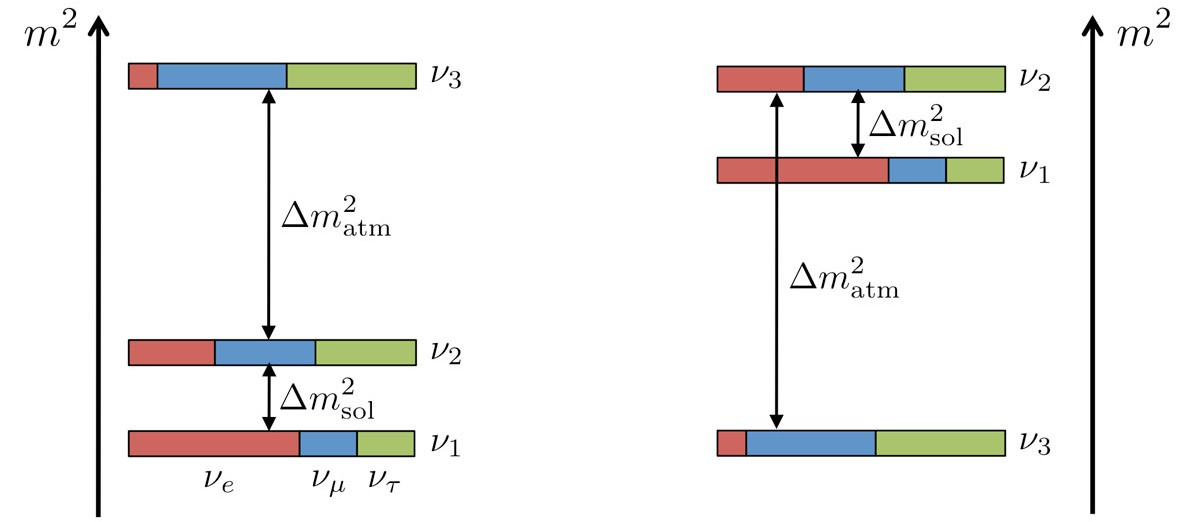
\includegraphics[width = 0.7\textwidth]{figures/mass-hierarchy.jpg}
    \caption{Representation of the two possible mass orderings: normal ordering on the left and inverted ordering on the right.
    The Figure specifies that $\Delta m^2_{21}$ is obtained via solar neutrinos measurements while $\Delta m^2_{32}$ 
    is given by atmospheric neutrinos experiments. Different colours refer to different neutrino flavours: red for the electron flavour, 
    blue for the muon one and green for the tau, respectively. Figure taken from \cite{fermilab-mass-ordering}.}
    \label{fig:mass-ordering}
\end{figure}


\subsection{The Seesaw mechanism}
\label{subsec:seesaw}
Experimental studies confirm that neutrinos do have masses, therefore there must be a corresponding mass term in the Lagrangian. 
Said term can be introduced in the same way as for the up-type quarks\footnote{Recalling the correspondence $u \rightarrow \nu$ and $d \rightarrow \ell$ in the SU(2)$_\text{L}$ doublets.}, using the conjugate Higgs field, yielding a Dirac mass term after the \ac{SSB} as expressed in Eq.~\ref{eq:neutrinos-dirac-masses}
\begin{equation}
    \label{eq:neutrinos-dirac-masses}
    \mathcal{L}_{D} = - m_D (\overline{\nu}_\text{R}\nu_\text{L} + \overline{\nu}_\text{L}\nu_\text{R}) = -\frac{1}{2}m_D (\overline{\nu_\text{L}}\nu_\text{R} + \overline{\nu_\text{R}^c}\nu_\text{L}^c) + \text{h.c.}
\end{equation}
where in the second part we used the equivalence $\overline{\nu_\text{L}}\nu_\text{R} \longleftrightarrow \overline{\nu_\text{R}^c}\nu_\text{L}^c $.
It is clear that if this is the origin of neutrino masses, then \ac{RH}\footnote{Unless otherwise specified, right and left refer to chiral states.}
neutrinos---and \ac{LH} antineutrinos as well---must exist. However, neutrino masses are much smaller than those of other fermions, either the charged leptons or the quarks for which masses arise in the Higgs mechanism, suggesting that there might be a different phenomenon which generates neutrino masses.

Seeing that \ac{RH} neutrinos and \ac{LH} antineutrinos transform as singlets under the \ac{SM} gauge group, any additional term formed by these fields can be added to the \ac{SM} Lagrangian without breaking its gauge invariance.

While \ac{RH} neutrinos appear as such in the new Lagrangian term, \ac{LH} antineutrinos are defined as the \ac{CP} conjugate fields of \ac{RH} neutrinos as written in Eq.~\ref{eq:CPconjugation-righHanded}
\begin{equation}
    \label{eq:CPconjugation-righHanded}
    \psi^c = \hat{C}\hat{P}\psi = i\gamma^2\gamma^0\psi^*.
\end{equation} 
Therefore in the Majorana mass term of Eq.~\ref{eq:neutrinos-majorana-masses}, \ac{LH} antineutrinos are written as $\nu_\text{R}^c$ yielding
\begin{equation}
    \label{eq:neutrinos-majorana-masses}
    \mathcal{L}_M = -\frac{1}{2} M \left( \overline{\nu_\text{R}^c} \nu_\text{R} + \overline{\nu_\text{R}} \nu_\text{R}^c \right).
\end{equation}
 

This term clearly respects the local gauge invariance of the \ac{SM}, and consequently it can be added to the \ac{SM} Lagrangian. 
It is now crucial to notice that the Majorana mass term provides a direct coupling between a particle and an antiparticle. 
Thus the corresponding Majorana mass term for the electron would allow $e^+ \leftrightarrow e^-$ transitions, violating charge conservation. 
This problem does not exist for the neutrinos. Nevertheless, seeing that neutrinos are neutral, it is possible that they are their own 
antiparticles, in which case they are referred to as \textit{Majorana neutrinos} and not as \textit{Dirac neutrinos}.

Finally, we can write the general mass Lagrangian for neutrinos including both Eqs.~\ref{eq:neutrinos-dirac-masses} 
and~\ref{eq:neutrinos-majorana-masses}, obtaining Eq.~\ref{eq:neutrinos-diracANDmajorana-masses}.
\begin{equation}
    \label{eq:neutrinos-diracANDmajorana-masses}
    \mathcal{L}_{DM} = -\frac{1}{2} \left[ m_D \overline{\nu_\text{L}}\nu_\text{R} + m_D \overline{\nu_\text{R}^c}\nu_\text{L}^c + M \overline{\nu_\text{R}^c}\nu_\text{R} \right] + \text{h.c.}
\end{equation}
The two different couplings can be represented using Feynman diagrams as depicted in Figure~\ref{fig:feynman-massCouplings}.
\begin{figure}[H]
    \centering
    \begin{tikzpicture}[
    thick,
    % Stile per i fermioni (linea continua con freccia a metà)
    fermion/.style={draw=black, postaction={decorate},
        decoration={markings, mark=at position 0.55 with {\arrow{latex}}}},
    % Stile per il campo scalare (linea tratteggiata)
    scalar/.style={draw=black, dashed},
    % Stile per la X
    cross/.style={cross out, draw=black, thick, minimum size=8pt, inner sep=0pt},
    % Stile per il vertice puntiforme
    dot/.style={circle, fill=black, minimum size=4pt, inner sep=0pt}
]

% ---------------- DIAGRAMMA DI DIRAC (Sinistra) ----------------
\coordinate (D) at (0,0);

% Linee entrante e uscente
\draw[fermion] (-1.5, 1.5) node[left] {$\nu_L$} -- (D);
\draw[fermion] (D) -- (1.5, 1.5) node[right] {$\nu_R$};

% Linea tratteggiata (Higgs) con la X finale
\draw[scalar] (D) -- (0, -1.5);
\node[cross] at (0, -1.5) {};

% Vertice centrale con pallino e label
\node[dot, label=right:{$m_D$}] at (D) {};


% ---------------- DIAGRAMMA DI MAJORANA (Destra) ----------------
\coordinate (M) at (6, 0.5); % Spostato a destra e leggermente in alto per allineamento visivo

% Linee (entrambe puntano verso il centro)
\draw[fermion] (4, 0.5) node[left] {$\nu_R$} -- (M);
\draw[fermion] (8, 0.5) node[right] {$\overline{\nu}_L$} -- (M);

% Vertice centrale con la X e label
\node[cross, label=above:{$M$}] at (M) {};

\end{tikzpicture}
    \caption{Feynman diagrams of the two possible mass couplings. On the left the Dirac coupling, associated with $m_D$. On the right the Majorana coupling, associated with $M$.}
    \label{fig:feynman-massCouplings}
\end{figure}

Eq.~\ref{eq:neutrinos-diracANDmajorana-masses} can be equivalently rewritten as Eq.~\ref{eq:neutrinos-diracANDmajorana-masses-matrix}
\begin{equation}
    \label{eq:neutrinos-diracANDmajorana-masses-matrix}
    \mathcal{L}_{DM} = -\frac{1}{2} \left( \overline{\nu_\text{L}} \quad \overline{\nu_\text{R}^c} \right) \underbrace{\begin{pmatrix} 0 & m_D \\ m_D & M \end{pmatrix}}_{\mathbf{M}} \begin{pmatrix} \nu_\text{L}^c \\ \nu_\text{R} \end{pmatrix} + \text{h.c.}
\end{equation}

where we identified the mass matrix $\mathbf{M}$, which can be diagonalised in order to define the physical states. 
The characteristic equation $\det(\mathbf{M} - \lambda \mathbb{1}) = 0$ yields $\lambda^2 - M\lambda - m_D^2 = 0$, 
from which one gets the masses of the physical neutrinos 
\begin{equation*}
    m_{\pm} = \lambda_{\pm} = \frac{M \pm \sqrt{M^2 + 4m_D^2}}{2} = \frac{M \pm M\sqrt{1 + 4m_D^2/M^2}}{2}.
\end{equation*}
Furthermore, taking the Majorana mass $M$ much greater than the Dirac mass $m_D$, 
i.e. $M \gg m_D$\footnote{The Dirac mass is assumed to be of the same order of the mass of the other fermions ($\mathcal{O}(1~\text{GeV})$), 
while the Majorana mass term is thought to be very large ($\mathcal{O}(10^{11}~\text{GeV})$) in order to get $m_\nu \sim 0.01$~eV.}, 
the two possible masses reduce to 
\begin{equation*}
    m_{\pm} \approx \frac{1}{2}M \pm \frac{1}{2}\left( M + \frac{2m_D^2}{M} \right)
\end{equation*}
giving a light neutrino state ($\nu$) and a heavy neutrino state ($N$) with the masses reported in Eq.~\ref{eq:final-nu-masses}
\begin{equation}
    \label{eq:final-nu-masses}
    |m_{\nu}| \approx \frac{m_D^2}{M} \quad \text{and} \quad m_N \approx M.
\end{equation} 
Therefore, if we go back to Eq.~\ref{eq:neutrinos-diracANDmajorana-masses-matrix}, we can rewrite $\nu$ and $N$ as a function of
$\nu_\text{L}$, $\nu_\text{L}^c$, $\nu_\text{R}$ and $\nu_\text{R}^c$ as shown in Eq.~\ref{eq:neutrinos-revisited}
\begin{equation}
    \label{eq:neutrinos-revisited}
    \nu = \cos\theta (\nu_\text{L} + \nu_\text{L}^c) - \sin\theta (\nu_\text{R} + \nu_\text{R}^c) \quad \text{and} \quad N = \cos\theta (\nu_\text{R} + \nu_\text{R}^c) + \sin\theta (\nu_\text{L} + \nu_\text{L}^c)
\end{equation}
where the mixing angle $\theta$ is determined by the ratio of the Dirac and Majorana masses, with $\theta = \frac{m_D}{M}$. 
Since the Majorana mass scale $M$ is assumed to be enormous compared to the Dirac mass, this ratio is extremely small. 
Consequently, $\theta$ tends to zero and this allows us to apply the small-angle approximations for the trigonometric functions such that
$\tan\theta \sim \theta \sim \frac{m_D}{M}~$ and consequently one gets $~\cos\theta \sim 1~$ and $~\sin\theta \sim \theta = \frac{m_D}{M}~$.\\
This consideration yields
\begin{equation*}
    \nu \approx (\nu_\text{L} + \nu_\text{L}^c) - \frac{m_D}{M}(\nu_\text{R} + \nu_\text{R}^c) ~ \text{and} ~ N \approx (\nu_\text{R} + \nu_\text{R}^c) + \frac{m_D}{M}(\nu_\text{L} + \nu_\text{L}^c).
\end{equation*}
It is now evident that the light-neutrino state is almost entirely \ac{LH} while the heavy-neutrino one is almost entirely \ac{RH}. 
Therefore, the latter participates neither in the weak \ac{CC} interactions nor in the weak \ac{NC} interactions of the \ac{SM}.

The process described so far, set against the Higgs mechanism for mass, is known as \textit{seesaw mechanism}.
It is only a hypothesis, but it would be more grounded if neutrinos were shown to be Majorana particles.
Their Majorana nature could be established by observing neutrinoless double $\beta$-decay, which is discussed in Section~\ref{sec:0nubetabeta}.
\chapter{Beta and double beta decay}
Beta decay is a nuclear transition in which a nucleus $(Z, A)$ converts into an isobar $(Z \pm 1, A)$ through the weak interaction, with the emission of an electron or positron and the corresponding (anti)neutrino, as anticipated in Chapter~\ref{chapter:nuIntro}. The single-beta decay process can be written as
\begin{equation}
    \label{eq:single-beta-decay}
    (Z, A) \longrightarrow (Z+1, A) + e^- + \overline{\nu}_e \qquad \text{or} \qquad 
    (Z, A) \longrightarrow (Z-1, A) + e^+ + \nu_e,
\end{equation}
depending on whether a neutron ($\beta^-$) or a proton ($\beta^+$) undergoes the weak transition. Enrico Fermi described this process in 1934~\cite{Fermi1934} by introducing a point-like, four-fermion contact interaction Hamiltonian
\begin{equation}
    H_F = G_F \left( \overline{\psi}_p \gamma^\mu \psi_n \right)\left( \overline{\psi}_e \gamma_\mu \psi_\nu \right) + \text{h.c.}
\end{equation} 
with $G_F$ the Fermi coupling constant, later reinterpreted within the \ac{SM} as the low-energy, effective limit of the \ac{CC} interaction (Eq.~\ref{eq:SM-neutrino-lagrangian}) where a virtual $W$ boson mediates, at the quark level, the $d \to u$ or $u \to d$ transitions. The process is allowed whenever it is energetically favourable, i.e. whenever its $Q$-value, given by the mass difference between the parent and daughter atoms, is positive. It is precisely this energy balance, together with nuclear pairing effects, that determines which nuclei undergo ordinary $\beta$ decay and which ones are instead only accessible through the second-order process of double-$\beta$ decay, discussed further in this Chapter.

\section{Two-neutrino double beta decay (\texorpdfstring{$2\nu\boldsymbol{\beta}\boldsymbol{\beta}$}{2vbb})}
\label{sec:2nubetabeta}
Double beta decay is a second-order weak interaction process in which a nucleus $(Z, A)$ decays directly into one of its isobars $(Z\pm2, A)$, changing its charge by two units while leaving the mass number unchanged. First proposed in 1935 by Maria Goeppert-Mayer~\cite{firstDoubleBeta}, it can be seen as the double counterpart of single-$\beta$ decay. Just as the latter comes in the $\beta^-$, $\beta^+$ and \ac{EC} variants, double beta decay with the emission of two neutrinos, $2\nu\beta\beta$, can proceed through four different modes: $\beta^-\beta^-$, $\beta^+\beta^+$, $\beta^+$\ac{EC} and \ac{EC}\ac{EC}, where in the last two the nucleus captures one or two electrons from the atomic shells. All of them perfectly conserve the lepton number and are fully accommodated within the \ac{SM}. They are summarised in Table~\ref{tab:bb-modes}.

\begin{table}[H]
    \centering
    \begin{tabular}{ll}
        \toprule
        \textbf{decay mode} & $\boldsymbol{2\nu}$ \textbf{channel} \\
        \midrule
        $\beta^-\beta^-$ & $(Z,A) \to (Z+2,A) + 2e^- + 2\overline{\nu}_e$ \\
        $\beta^+\beta^+$ & $(Z,A) \to (Z-2,A) + 2e^+ + 2\nu_e$ \\
        $\beta^+$\ac{EC} & $e^-_\text{b} + (Z,A) \to (Z-2,A) + e^+ + 2\nu_e$ \\
        \ac{EC}\ac{EC} & $2e^-_\text{b} + (Z,A) \to (Z-2,A) + 2\nu_e$ \\
        \bottomrule
    \end{tabular}
    \caption{Possible modes of $2\nu\beta\beta$ decay. $e^-_\text{b}$ denotes an electron captured from the atomic shell.}
    \label{tab:bb-modes}
\end{table}

The energy conditions differ from mode to mode. Working with atomic masses, the $\beta^-\beta^-$ decay only requires $M(Z,A) > M(Z+2,A)$. For the modes that decrease the nuclear charge, the mass difference $M(Z,A) - M(Z-2,A)$ must instead exceed $2m_ec^2 \simeq 1022$~keV for $\beta^+$\ac{EC} and $4m_ec^2 \simeq 2044$~keV for $\beta^+\beta^+$, since each emitted positron costs $2m_ec^2$, while the \ac{EC}\ac{EC} mode has no such penalty. In addition, the Coulomb repulsion between the nucleus and the positron further suppresses positron emission. As a result, the modes involving $\beta^+$ and \ac{EC} generally have low effective $Q$-values and rates much smaller than $\beta^-\beta^-$, and are usually neglected. In principle, each of these modes could also occur without the emission of neutrinos, a lepton-number-violating process discussed in Section~\ref{sec:0nubetabeta}. 

Seeing that this work focuses on ${}^{76}$Ge double-beta decay, in what follows $\beta\beta$ refers to the $\beta^-\beta^-$ mode detailed in the first row of Table~\ref{tab:bb-modes}.

At the microscopic level, the process occurs through two simultaneous, virtual single-$\beta$ transitions, as illustrated by the two weak vertices in the Feynman diagram of Figure~\ref{fig:2nu_feynman}.

\begin{figure}[H]
    \centering
    \begin{center}
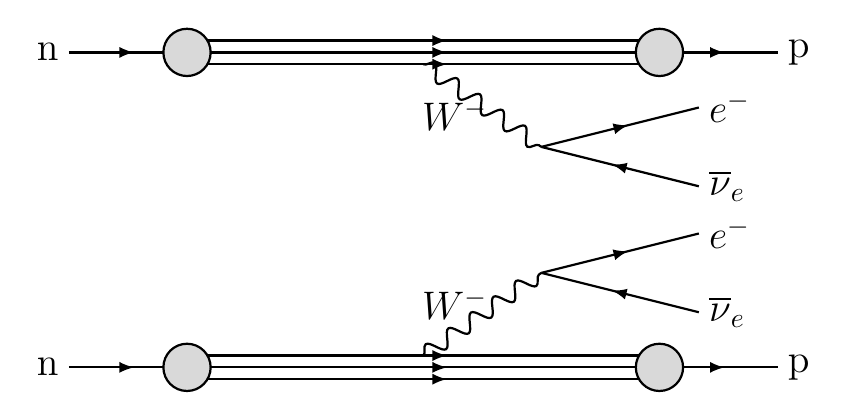
\begin{tikzpicture}[
    thick,
    % Stile per le linee dei fermioni (linea con freccia a metà)
    fermion/.style={draw=black, postaction={decorate},
        decoration={markings, mark=at position 0.55 with {\arrow{latex}}}},
    % Stile per i bosoni W (linea ondulata)
    boson/.style={draw=black, decorate,
        decoration={snake, amplitude=1mm, segment length=3.5mm}},
    % Stile per i vertici dei nucleoni (i cerchi grigi)
    blob/.style={circle, draw=black, fill=gray!30, minimum size=6mm, inner sep=0pt}
]

% ---------------- NUCLEONE SUPERIORE ----------------
% Frecce esterne n e p
\draw[fermion] (-4.5, 2) node[left, font=\Large] {n} -- (-3, 2);
\draw[fermion] (3, 2) -- (4.5, 2) node[right, font=\Large] {p};

% Le 3 linee dei quark all'interno (tra i due blob)
\draw[fermion] (-3, 2.15) -- (3, 2.15);
\draw[fermion] (-3, 2.0) -- (3, 2.0);
\draw[fermion] (-3, 1.85) -- (3, 1.85);

% Bosone W- 
\draw[boson] (0, 1.85) -- (1.5, 0.8);
\node[font=\Large] at (0.4, 1.2) {$W^-$};

% Elettrone e antineutrino 
% (Nota: la linea del neutrino è disegnata da destra a sinistra per invertire la freccia)
\draw[fermion] (1.5, 0.8) -- (3.5, 1.3) node[right, font=\Large] {$e^-$};
\draw[fermion] (3.5, 0.3) node[right, font=\Large] {$\overline{\nu}_e$} -- (1.5, 0.8);


% ---------------- NUCLEONE INFERIORE ----------------
% Frecce esterne n e p
\draw[fermion] (-4.5, -2) node[left, font=\Large] {n} -- (-3, -2);
\draw[fermion] (3, -2) -- (4.5, -2) node[right, font=\Large] {p};

% Le 3 linee dei quark all'interno (tra i due blob)
\draw[fermion] (-3, -1.85) -- (3, -1.85);
\draw[fermion] (-3, -2.0) -- (3, -2.0);
\draw[fermion] (-3, -2.15) -- (3, -2.15);

% Bosone W- 
\draw[boson] (0, -1.85) -- (1.5, -0.8);
\node[font=\Large] at (0.4, -1.2) {$W^-$};

% Elettrone e antineutrino
\draw[fermion] (1.5, -0.8) -- (3.5, -0.3) node[right, font=\Large] {$e^-$};
\draw[fermion] (3.5, -1.3) node[right, font=\Large] {$\overline{\nu}_e$} -- (1.5, -0.8);


% --- DISEGNO I BLOB ---
% (Disegnati per ultimi così coprono perfettamente le estremità delle linee)
\node[blob] at (-3, 2) {};
\node[blob] at (3, 2) {};
\node[blob] at (-3, -2) {};
\node[blob] at (3, -2) {};

\end{tikzpicture}
\end{center}
    \caption{Feynman diagram of $2\nu\beta\beta$. The process proceeds via the exchange of two virtual $W^-$ bosons, resulting in the simultaneous emission of two electrons and two electron antineutrinos.}
    \label{fig:2nu_feynman}
\end{figure}

\begin{wrapfigure}{l}{0.52\textwidth}%[H]
    \centering
    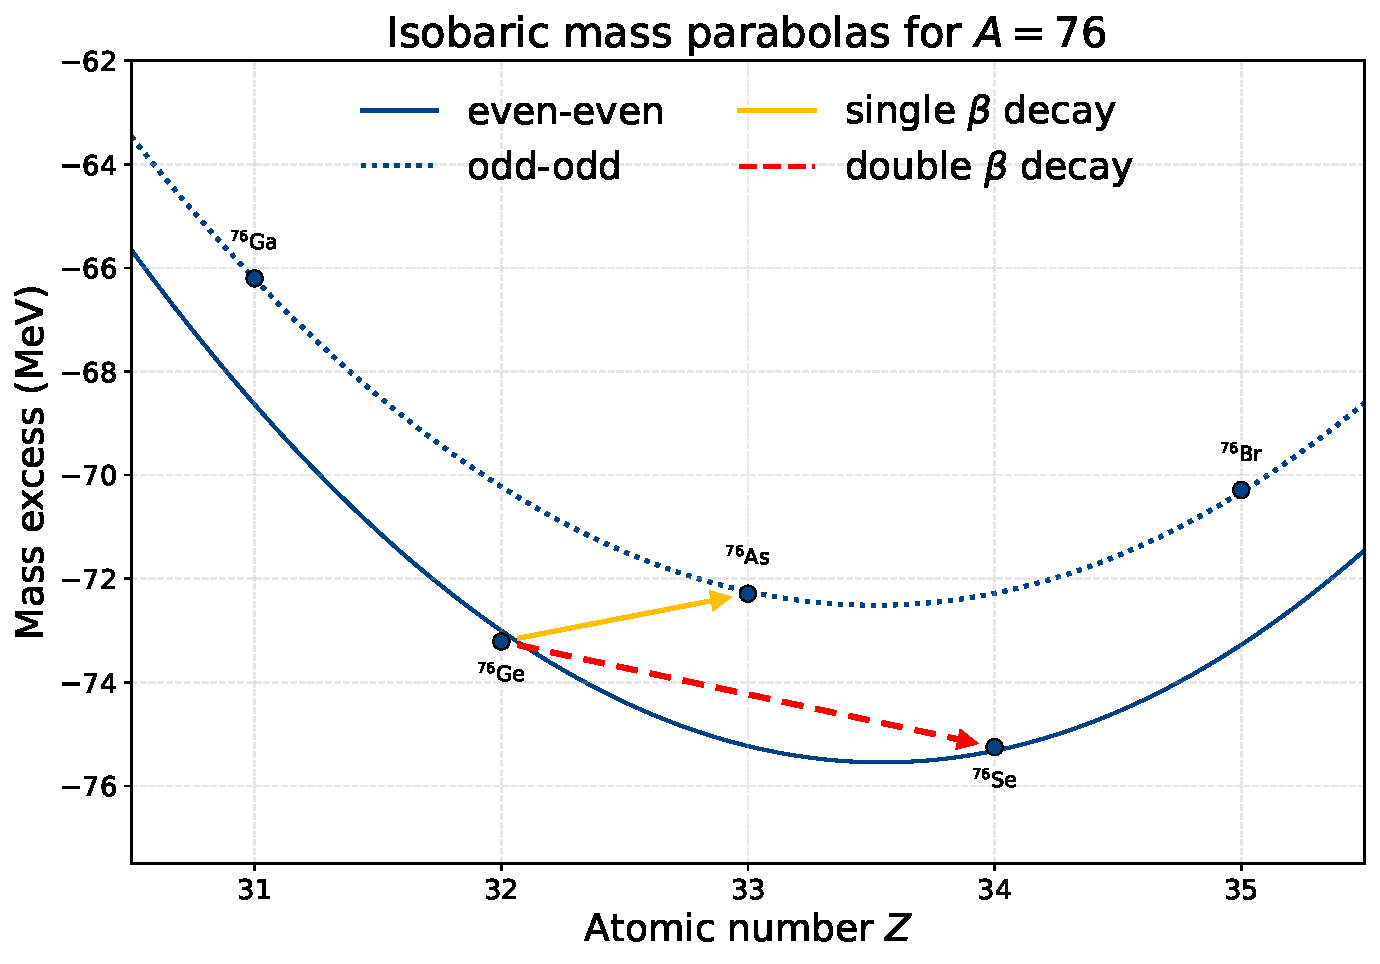
\includegraphics[width=\linewidth]{figures/mass_parabola_A76.pdf}
    \caption{Mass parabolas for $A=76$ isobars. A detailed description is given in the text. Custom plot with data taken from \cite{AME2020-masses} and \cite{Ge76-Qvalue}.}
    \label{fig:doublebeta-parabola}
\end{wrapfigure}
For a nucleus to undergo such a rare decay, the standard single-$\beta$ decay to the intermediate isobar $(Z+1, A)$ must be energetically forbidden or heavily suppressed. This kinematic condition naturally arises in even-even nuclei due to the nuclear pairing interaction, which binds them more tightly than their odd-odd neighbours. As a consequence, while the direct transition $(Z, A) \to (Z+1, A)$ is blocked, the target state $(Z+2, A)$ still sits at a lower energy level, effectively opening the double-$\beta$ channel. 
This energy landscape is visualised using mass parabolas, as shown in Figure~\ref{fig:doublebeta-parabola} for the case of ${}^{76}\text{Ge}$, where the even-even and odd-odd mass parabolas are shown with a continuous and dashed line, respectively. The double-beta transition of ${}^{76}\text{Ge}$ is highlighted in red, while the yellow lines represent ordinary single-$\beta$ decays. The intermediate odd-odd state acts as a virtual state in the quantum mechanical transition and is never physically populated.

Because $2\nu\beta\beta$ is a second-order process in the weak coupling, its decay rate is massively suppressed compared to ordinary $\beta$ decay, resulting in extremely long half-lives of the order of $T_{1/2}^{2\nu} \sim 10^{19}$--$10^{24}$~years, depending on the isotope.

Unlike the neutrinoless mode, $2\nu\beta\beta$ does not require any new physics beyond the \ac{SM} and has been experimentally observed in about 10 different even-even isotopes. Nuclei such as ${}^{76}\text{Ge}$ are of particular relevance in modern physics, as they also represent the most promising candidates in the search for neutrinoless double beta decay, a process that violates lepton number by two units and is discussed in detail in Section~\ref{sec:0nubetabeta}.

\section{Neutrinoless double beta decay (\texorpdfstring{$0\nu\boldsymbol{\beta}\boldsymbol{\beta}$}{0vbb})}
\label{sec:0nubetabeta}

In Section~\ref{sec:2nubetabeta}, $2\nu\beta\beta$ was introduced as a rare second-order weak process, allowed by the \ac{SM} because it conserves lepton number. Neutrinoless double-$\beta$ decay ($0\nu\beta\beta$) differs from it by a single, but crucial, feature: no (anti)neutrino is present in the final state, so that the processes of Table~\ref{tab:bb-modes} are to be rewritten as in Table~\ref{tab:0nubb-modes}.


\begin{table}[H]
    \centering
    \begin{tabular}{ll}
        \toprule
        \textbf{decay mode} & $\boldsymbol{0\nu}$ \textbf{channel} \\
        \midrule
        $\beta^-\beta^-$ & $(Z,A) \to (Z+2,A) + 2e^-$\\
        $\beta^+\beta^+$ & $(Z,A) \to (Z-2,A) + 2e^+$\\
        $\beta^+$\ac{EC} & $e^-_\text{b} + (Z,A) \to (Z-2,A) + e^+$ \\
        \ac{EC}\ac{EC} & $2e^-_\text{b} + (Z,A) \to (Z-2,A)$\\
        \bottomrule
    \end{tabular}
    \caption{Possible modes of $0\nu\beta\beta$ decay. $e^-_\text{b}$ denotes an electron captured from the atomic shell.}
    \label{tab:0nubb-modes}
\end{table}


This implies a violation of lepton number by two units ($\Delta L=2$), which is forbidden in the \ac{SM}. Its observation would therefore be a clear signal of physics beyond the \ac{SM}, with several implications. Since the decay can be mediated by different mechanisms (e.g.\ the exchange of a light Majorana neutrino, of heavy particles or right-handed currents~\cite{review-0nu-2015}), these implications can be divided into two groups: those that do not depend on the mediating mechanism, and those that hold only under specific assumptions on it.

\begin{enumerate}
\item \textbf{model-independent consequences}:
\begin{itemize}
    \item \textit{matter creation}: it would be the first laboratory observation of a process that produces matter without producing the corresponding antimatter.
    \item \textit{violation of lepton number and of $B-L$}: since the baryon number $B$ is not affected by the decay, a $\Delta L = 2$ process also violates $B-L$. This would be the first experimental evidence that such a symmetry, which is only accidental in the \ac{SM} and has no theoretical reason to be exact, is broken in nature.
    \item \textit{Majorana nature of neutrinos}: whatever the underlying mechanism, an observed $0\nu\beta\beta$ decay implies that neutrinos can convert into antineutrinos, hence that they are Majorana particles.
\end{itemize}

\item \textbf{model-dependent consequences}: if the decay is dominated by the exchange of a light Majorana neutrino, the measured half-life can be translated into a value of the effective Majorana mass $m_{\beta\beta}$ (see Eq.~\ref{eq:half-life_0nubb} below), which gives access to:
\begin{itemize}
    \item \textit{absolute neutrino mass scale}: oscillation experiments are sensitive only to mass-squared differences, while combining $m_{\beta\beta}$ with direct measurements from single $\beta$ decay and with cosmological data allows one to constrain the individual mass eigenvalues (central and right panels of Fig.~\ref{fig:mbb_allowed});
    \item \textit{mass ordering}: comparing $m_{\beta\beta}$ with the regions allowed for the normal and inverted ordering (Fig.~\ref{fig:mbb_allowed}), the ordering could be established. In the inverted case $m_{\beta\beta}$ is bounded from below, while in the normal one it can vanish. If $m_{\beta\beta}$ falls where the two regions overlap, the ordering can be established only by combining it with an independent measurement of the mass scale, through $m_\beta$ or $\Sigma$.
\end{itemize}
\end{enumerate} 

The model-independent results are also relevant for cosmology. The Universe appears to contain only matter, and the \ac{SM} cannot account for the observed matter-antimatter asymmetry: although it contains sources of $CP$ and baryon-number violation, two of the conditions identified by Sakharov~\cite{sakharov}, they are too weak to generate it. A new source of violation of global symmetries is therefore needed, and leptogenesis models provide it: a lepton asymmetry is generated through lepton-number-violating processes and then partially converted into a baryon asymmetry. Observing $0\nu\beta\beta$ would support this class of scenarios~\cite{morella}.


As established earlier, this work centres on ${}^{76}\text{Ge}$. Hereafter, we consider exclusively the light-neutrino exchange channel for its neutrinoless decay, formulated in Eq.~\ref{eq:0nu-beta-beta} and represented in Figure~\ref{fig:0nubetabeta-diagram}.

\begin{equation}
    \label{eq:0nu-beta-beta}
    (Z, A) \longrightarrow (Z+2, A) + 2e^-
\end{equation} 

\begin{figure}[H]
    \centering
    \begin{center}
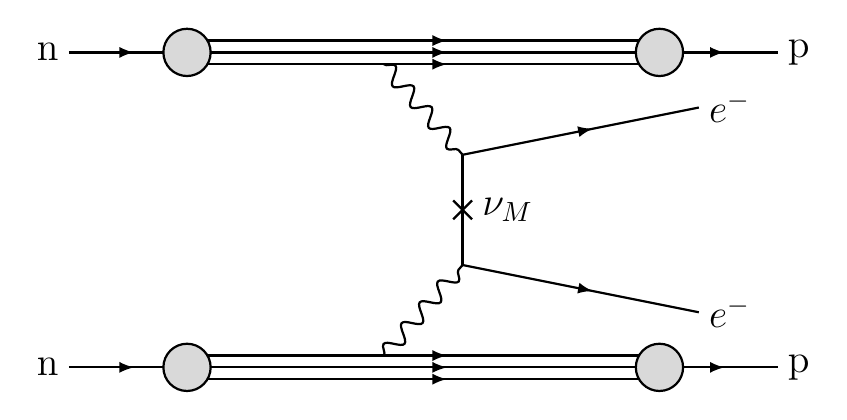
\begin{tikzpicture}[
    thick,
    % Stile per le linee dei fermioni (linea con freccia a metà)
    fermion/.style={draw=black, postaction={decorate},
        decoration={markings, mark=at position 0.55 with {\arrow{latex}}}},
    % Stile per i bosoni W (linea ondulata)
    boson/.style={draw=black, decorate,
        decoration={snake, amplitude=1mm, segment length=3.5mm}},
    % Stile per la massa di Majorana (la X al centro)
    cross/.style={cross out, draw=black, thick, minimum size=6pt, inner sep=0pt},
    % Stile per i vertici dei nucleoni (i cerchi grigi)
    blob/.style={circle, draw=black, fill=gray!30, minimum size=6mm, inner sep=0pt}
]

% ---------------- NUCLEONE SUPERIORE ----------------
\draw[fermion] (-4.5, 2) node[left, font=\Large] {n} -- (-3, 2);
\draw[fermion] (3, 2) -- (4.5, 2) node[right, font=\Large] {p};

\draw[fermion] (-3, 2.15) -- (3, 2.15);
\draw[fermion] (-3, 2.0) -- (3, 2.0);
\draw[fermion] (-3, 1.85) -- (3, 1.85);

% ---------------- NUCLEONE INFERIORE ----------------
\draw[fermion] (-4.5, -2) node[left, font=\Large] {n} -- (-3, -2);
\draw[fermion] (3, -2) -- (4.5, -2) node[right, font=\Large] {p};

\draw[fermion] (-3, -1.85) -- (3, -1.85);
\draw[fermion] (-3, -2.0) -- (3, -2.0);
\draw[fermion] (-3, -2.15) -- (3, -2.15);

% --- DISEGNO I BLOB ---
\node[blob] at (-3, 2) {};
\node[blob] at (3, 2) {};
\node[blob] at (-3, -2) {};
\node[blob] at (3, -2) {};

% ---------------- SCAMBIO INTERNO ----------------
% Bosoni W
\draw[boson] (-0.5, 1.85) -- (0.5, 0.7);
\draw[boson] (-0.5, -1.85) -- (0.5, -0.7);

% Neutrino di Majorana (dritto, senza freccia, con la X)
\draw (0.5, 0.7) -- (0.5, -0.7);
\node[cross, label={[font=\Large]right:{$\nu_M$}}] at (0.5, 0) {};

% Elettroni uscenti
\draw[fermion] (0.5, 0.7) -- (3.5, 1.3) node[right, font=\Large] {$e^-$};
\draw[fermion] (0.5, -0.7) -- (3.5, -1.3) node[right, font=\Large] {$e^-$};

\end{tikzpicture}
\end{center}
    \caption{Feynman diagram for neutrinoless double $\beta$-decay. The Majorana coupling of the neutrino with its own antineutrino (see Figure~\ref{fig:feynman-massCouplings}) is shown.}
    \label{fig:0nubetabeta-diagram}
\end{figure}


\begin{wrapfigure}{l}{0.52\textwidth}%[H]
    \centering
    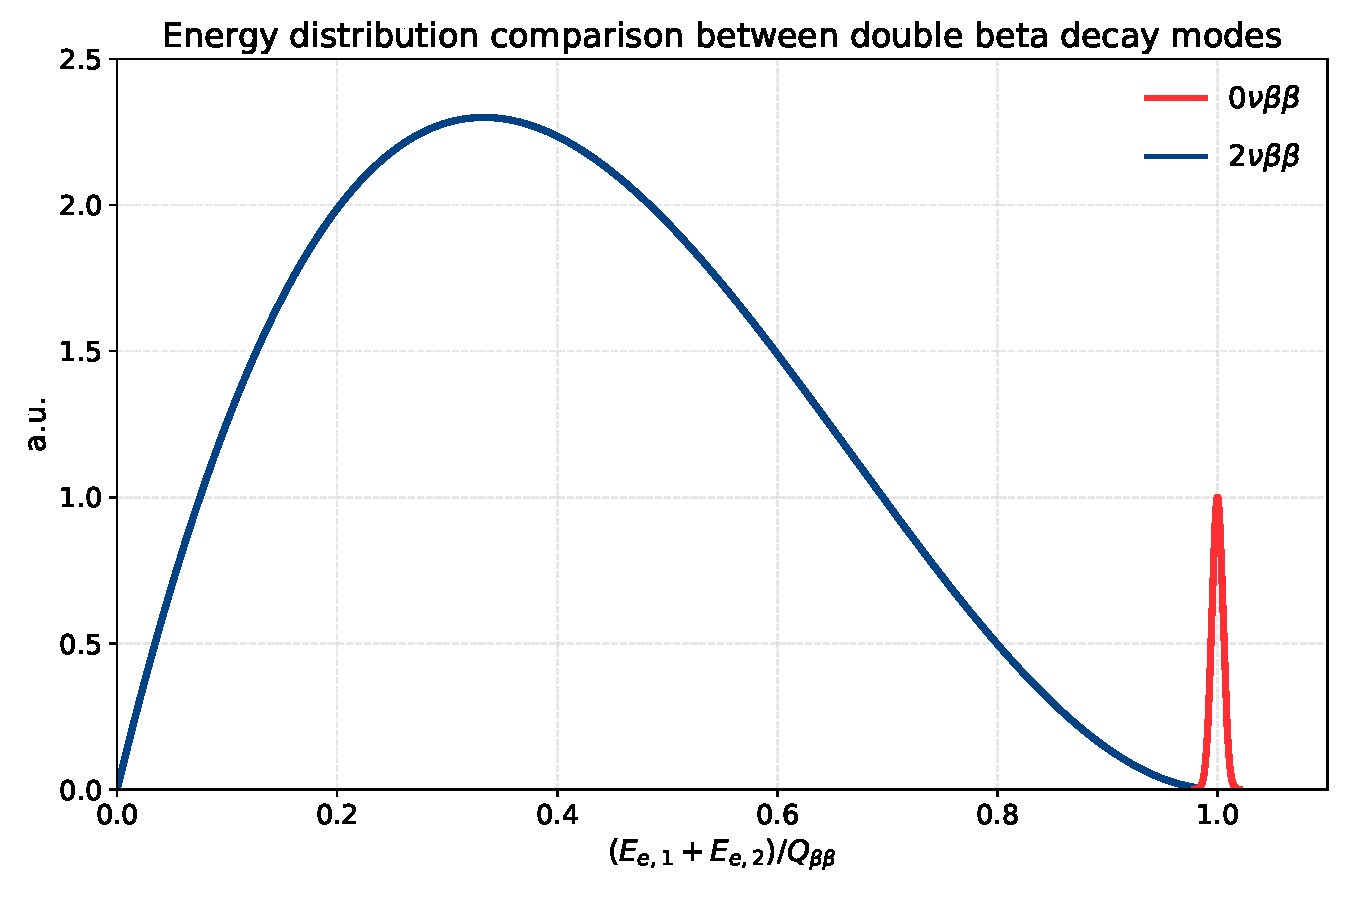
\includegraphics[width=\linewidth]{figures/0nu_vs_2nu.pdf}
    \caption{Schematic representation of the energy distribution for the products in $2\nu\beta\beta$ and $0\nu\beta\beta$ decay modes. The description is given in the text.}
    \label{fig:Qvalue-2nu0nu}
\end{wrapfigure}
From an experimental point of view, $0\nu\beta\beta$ can be distinguished from the more common $2\nu\beta\beta$ decay by analysing the energy spectrum of the two emitted electrons. Specifically, in $0\nu\beta\beta$ decay, the electrons are produced with energies $E_{e, 1}$ and $E_{e, 2}$ that satisfy
\begin{equation*}
    E_{e, 1} + E_{e, 2} + E_{\text{nuc}} = Q_{\beta\beta} = M(Z, A) - M(Z+2, A)
\end{equation*}
where $M(Z, A)$ and $M(Z+2, A)$ are the atomic masses of the parent and daughter atoms, respectively. Since the energy of the recoiling nucleus is negligible, the sum of the electron energies equals the $Q$-value of the transition, i.e. $E_{e, 1} + E_{e, 2} = Q_{\beta\beta}$. Conversely, in standard $2\nu\beta\beta$ decay part of the energy is carried away by the two antineutrinos, so the summed electron energy has a continuous spectrum that extends up to $Q_{\beta\beta}$, with a maximum around one third of $Q_{\beta\beta}$ and very few events close to the endpoint. Fig.~\ref{fig:Qvalue-2nu0nu} shows this continuous spectrum in blue for the $2\nu\beta\beta$ process and the monoenergetic peak\footnote{The signal has ideally a Dirac delta signature but is represented here as a very narrow Gaussian because what would be eventually observed is limited by detector resolution.} at $Q_{\beta\beta}$ for $0\nu\beta\beta$ in red.

If neutrinos are indeed Majorana particles and the standard mechanism for $0\nu\beta\beta$ decay is mediated by the exchange of a light Majorana neutrino, the decay rate, usually expressed in terms of the half-life $T_{1/2}^{0\nu}$, is given by:
\begin{equation}
    \label{eq:half-life_0nubb}
    (T_{1/2}^{0\nu})^{-1} = G_{0\nu}(Q_{\beta\beta}, Z) \left| \mathcal{M}_{0\nu} \right|^2 \left( \frac{m_{\beta\beta}}{m_e} \right)^2
\end{equation}
where $G_{0\nu}(Q_{\beta\beta}, Z)$ is the phase space factor, which depends on the $Q$-value and on the atomic number $Z$, $\mathcal{M}_{0\nu}$ is the nuclear matrix element, $m_e$ is the electron mass, and $m_{\beta\beta} = \big|\sum_{i=1}^{3} U_{ei}^2\, m_i\big|$ denotes the effective Majorana mass. The latter depends on the elements of the first row of $U_\text{PMNS}^\text{Maj}$, including the Majorana phases, and on the neutrino mass eigenvalues; through $m_{\beta\beta}$, the decay rate is therefore also sensitive to the \ac{NMO}.

Using the parametrisation of Eqs.~\ref{eq:Upmns-majorana} and~\ref{eq:Upmns-total}, the effective Majorana mass can be written explicitly as
\begin{equation}
  m_{\beta\beta} = \left| c_{12}^2 c_{13}^2\, m_1 + s_{12}^2 c_{13}^2\, m_2\, e^{i\alpha_{21}} + s_{13}^2\, m_3\, e^{i(\alpha_{31}-2\delta)} \right| .
  \label{eq:mbb_explicit}
\end{equation}
Mixing angles and mass-squared differences are measured by oscillation experiments, but $m_{\beta\beta}$ also depends on three quantities they cannot access: the two Majorana phases and the absolute mass scale. For a given mass scale, letting the phases vary between the values that maximise and minimise $m_{\beta\beta}$ defines its allowed range. The mass scale can be expressed through the lightest neutrino mass $m_\text{light}$ ($m_1$ for normal and $m_3$ for inverted ordering), through the effective electron-neutrino mass measured in single $\beta$ decay, $m_\beta = \big(\sum_i |U_{ei}|^2 m_i^2\big)^{1/2}$, or through the sum of the masses constrained by cosmology, $\Sigma = \sum_i m_i$. The resulting regions are shown in Fig.~\ref{fig:mbb_allowed}.

At large mass scales the three neutrinos are quasi-degenerate and the two orderings overlap, while at lower values they separate. In the inverted ordering the two dominant terms of Eq.~\ref{eq:mbb_explicit} cannot cancel, since $\cos 2\theta_{12} \neq 0$, so $m_{\beta\beta}$ is bounded from below at about 18~meV~\cite{plot-esperiments_and_exposures}: next-generation experiments such as LEGEND-1000 aim to probe this whole region. In the normal ordering, instead, the three terms can cancel for $m_\text{light}$ of a few meV, and $m_{\beta\beta}$ can be arbitrarily small. Oscillation data also set a minimum value of $\Sigma$, about 59~meV for normal and 100~meV for inverted ordering, which is where the two regions start in the right panel.

\begin{figure}[H]
  \centering
  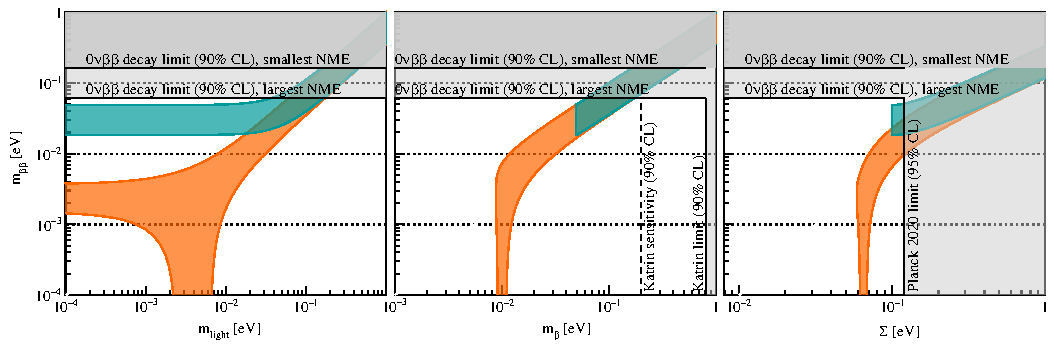
\includegraphics[width=\textwidth]{figures/mbb_NO_IO_Agostini2023.pdf}
  \caption[Allowed range of $m_{\beta\beta}$ as a function of $m_\text{light}$, $m_\beta$ and $\Sigma$]{%
  Range of $m_{\beta\beta}$ allowed by light Majorana neutrino exchange as a function of the lightest neutrino mass $m_\text{light}$ (left), of the effective electron-neutrino mass $m_\beta$ (centre) and of the sum of the neutrino masses $\Sigma$ (right), for normal (orange) and inverted (teal) ordering. The oscillation parameters are fixed to their central values, so the width of each region is due only to the unknown Majorana phases. Grey areas are excluded by $0\nu\beta\beta$ searches (KamLAND-Zen, 2016; the two horizontal lines correspond to the largest and smallest nuclear matrix element), by KATRIN (central panel) and by Planck (right panel); the dashed line in the central panel is the KATRIN design sensitivity. Limits are those available in 2023 (see text for updates). Figure taken from~\cite{plot-esperiments_and_exposures}.}
  \label{fig:mbb_allowed}
\end{figure}

The limits shown in Fig.~\ref{fig:mbb_allowed} reflect the status in 2023 and have since improved: KamLAND-Zen now sets $T_{1/2}^{0\nu} > 3.8\times10^{26}$~yr (Table~\ref{tab:0nubb-limits}), while the KATRIN and cosmological bounds have become $m_\beta < 0.45$~eV~\cite{katrin2025} and $\Sigma < 0.064$~eV~\cite{desi2025}, as anticipated in Section~\ref{subsec:NMO}. The cosmological bound, obtained by combining DESI DR2 and CMB data within $\Lambda$CDM, is already in tension with the minimum value allowed by oscillations, and relaxes to 0.163~eV if the dark energy equation of state is allowed to evolve~\cite{desi2025}.

Experimentally, observing $0\nu\beta\beta$ decay requires identifying a tiny, mono-energetic signal at $Q_{\beta\beta}$, so the choice of the best isotope to search for such a rare decay is the first issue to face, since it involves background suppression and energy resolution considerations, but also the limited time for which an experiment can be run. These considerations translate into a series of criteria for choosing a suitable isotope, which restrict the choice to elements with high isotopic abundance, a good compatibility with detection techniques and a sufficiently high $Q_{\beta\beta}$. The $Q$-values of the candidate isotopes span from about $2$~MeV up to a few MeV, a range where the dominant background is the environmental radioactivity of the natural ${}^{232}$Th and ${}^{238}$U decay chains, together with cosmic rays. Since the intensity of this background decreases with increasing energy, isotopes with a high enough $Q_{\beta\beta}$ are preferred, so that the region of interest lies where the background is lowest. To give an idea of the energy scale, natural $\gamma$ radioactivity extends up to the $2615$~keV line of ${}^{208}$Tl, the $\beta$ decay of ${}^{214}$Bi, from the ${}^{238}$U chain, reaches $3270$~keV, and $\alpha$ decays are even more energetic, around $5$~MeV (e.g. $5.3$~MeV for ${}^{210}$Po)~\cite{review-0nu-2015}.

Thus, the commonly studied isotopes are the ones listed in Table~\ref{tab:isotopes-for-0nu}, together with their isotopic abundance and $Q_{\beta\beta}$ values. ${}^{76}$Ge is an exception among them, since its $Q_{\beta\beta} = 2039$~keV lies in a region where natural $\gamma$ radioactivity is still present, which is in principle a limitation for background reduction. It is nevertheless one of the most studied isotopes, thanks to the excellent energy resolution and radiopurity of high-purity germanium detectors, in which the source coincides with the detector.

\begin{table}[H]
    \centering
    \begin{tabular}{lcc}
        \toprule
        Isotope & Isotopic abundance (\%) & $Q_{\beta\beta}$ [keV] \\
        \midrule
        ${}^{48}\text{Ca}$  & 0.187 & 4263 \\
        ${}^{76}\text{Ge}$  & 7.8   & 2039 \\
        ${}^{82}\text{Se}$  & 9.2   & 2998 \\
        ${}^{96}\text{Zr}$  & 2.8   & 3348 \\
        ${}^{100}\text{Mo}$ & 9.6   & 3035 \\
        ${}^{116}\text{Cd}$ & 7.6   & 2813 \\
        ${}^{130}\text{Te}$ & 34.08 & 2527 \\
        ${}^{136}\text{Xe}$ & 8.9   & 2459 \\
        ${}^{150}\text{Nd}$ & 5.6   & 3371 \\
        \bottomrule
    \end{tabular}
    \caption{Candidate isotopes for $0\nu\beta\beta$ search: isotopic abundance and $Q_{\beta\beta}$ value. Data are taken from \cite{review-0nu-2015}.}
    \label{tab:isotopes-for-0nu}
\end{table}

If a $0\nu\beta\beta$ signal is detected, its half-life can be experimentally evaluated as 
\begin{equation}
    \label{eq:half-life_0nubb_exp}
    T_{1/2}^{0\nu} = \ln(2) \cdot T \cdot \varepsilon \cdot \frac{N_{\beta\beta}}{N_\text{peak}}
\end{equation}
where $T$ is the measuring time, $\varepsilon$ is the detection efficiency, $N_{\beta\beta}$ is the number of $\beta\beta$-decaying nuclei under observation and $N_\text{peak}$ is the number of observed decays in the region of interest. If no peak is detected, the sensitivity of a given experiment is expressed in terms of a detector \textit{figure of merit} $S^{0\nu}$, i.e. the half-life corresponding to the maximum signal that could be hidden by the background fluctuations $n_{B}$. From Eq.~\ref{eq:half-life_0nubb_exp}, the sensitivity can be written as
\begin{equation}
    \label{eq:sensitivity-0nu}
    \begin{aligned}
        S^{0\nu} &= \ln 2 \cdot T \cdot \varepsilon \cdot \frac{N_{\beta\beta}}{n_\sigma \cdot n_B} \\
                 &= \ln 2 \cdot \varepsilon \cdot \frac{1}{n_\sigma} \cdot \frac{x\,\eta\,N_A}{\mathcal{M}_A} \cdot \sqrt{\frac{M \cdot T}{B \cdot \Delta E}},
    \end{aligned}
\end{equation}
where $n_\sigma$ is the confidence level in units of standard deviations and $n_B = \sqrt{B \cdot M \cdot T \cdot \Delta E}$ is the fluctuation of the number of background events in the region of interest~\cite{review-0nu-2015}. The exposure $M \cdot T$ is the product of detector mass and measuring time, $B$ is the background index, i.e. the background rate per unit mass, energy and time, and $\Delta E$ is the energy resolution (FWHM) at $Q_{\beta\beta}$. Finally, the second line follows from writing $N_{\beta\beta} = x\,\eta\,N_A\,M/\mathcal{M}_A$, where $x$ is the stoichiometric multiplicity of the candidate element in the compound, $\eta$ its isotopic abundance, $N_A$ Avogadro's number and $\mathcal{M}_A$ the molar mass of the compound.

This formula dictates the design of modern experiments: to maximise sensitivity, one must increase the exposure while minimising both the background level and the energy resolution. Specifically, a poor energy resolution causes the continuous tail of the standard $2\nu\beta\beta$ decay to smear into the $0\nu\beta\beta$ region of interest, creating an irreducible background.


\section{Experiments currently searching for \texorpdfstring{$0\nu\boldsymbol{\beta}\boldsymbol{\beta}$}{0nu beta beta} decay}
\label{sec:0nubb-experiments}
The experimental approach to $0\nu\beta\beta$ searches is based on the development of a detection technique able to balance good energy resolution, very low background and large isotope mass. Up to now, experiments in this field rely on two different techniques: calorimetric detectors, in which the source is embedded inside the detector volume itself, and detectors exploiting an external source~\cite{review-0nu-2015}. 

The best limits obtained so far for each candidate isotope are reported in Table~\ref{tab:0nubb-limits}~\cite{PDG:2026}, while the experiments currently running or planned, together with their expected sensitivities, are summarised in Fig.~\ref{fig:experiments-and-sensitivities-0nubb}.
\begin{table}[H]
    \centering
    \begin{tabular}{llc}
        \toprule
        Isotope & Experiment & $T_{1/2}^{0\nu}$ limit [yr] \\
        \midrule
        ${}^{48}\text{Ca}$  & CaF$_2$ scintillators     & $> 5.8 \times 10^{22}$ \\
        ${}^{76}\text{Ge}$  & GERDA + MJD + LEGEND-200  & $> 1.9 \times 10^{26}$ \\
        ${}^{82}\text{Se}$  & CUPID-0                   & $> 4.6 \times 10^{24}$ \\
        ${}^{96}\text{Zr}$  & NEMO-3                    & $> 9.2 \times 10^{21}$ \\
        ${}^{100}\text{Mo}$ & AMoRE-I                   & $> 2.9 \times 10^{24}$ \\
        ${}^{116}\text{Cd}$ & AURORA                    & $> 2.2 \times 10^{23}$ \\
        ${}^{130}\text{Te}$ & CUORE                     & $> 3.5 \times 10^{25}$ \\
        ${}^{136}\text{Xe}$ & KamLAND-Zen               & $> 3.8 \times 10^{26}$ \\
        ${}^{150}\text{Nd}$ & NEMO-3                    & $> 2.0 \times 10^{22}$ \\
        \bottomrule
    \end{tabular}
    \caption{Best current lower limits (90\% CL) on the $0\nu\beta\beta$ half-life for each candidate isotope \cite{PDG:2026}.}
    \label{tab:0nubb-limits}
\end{table}

\begin{figure}[H]
    \centering
    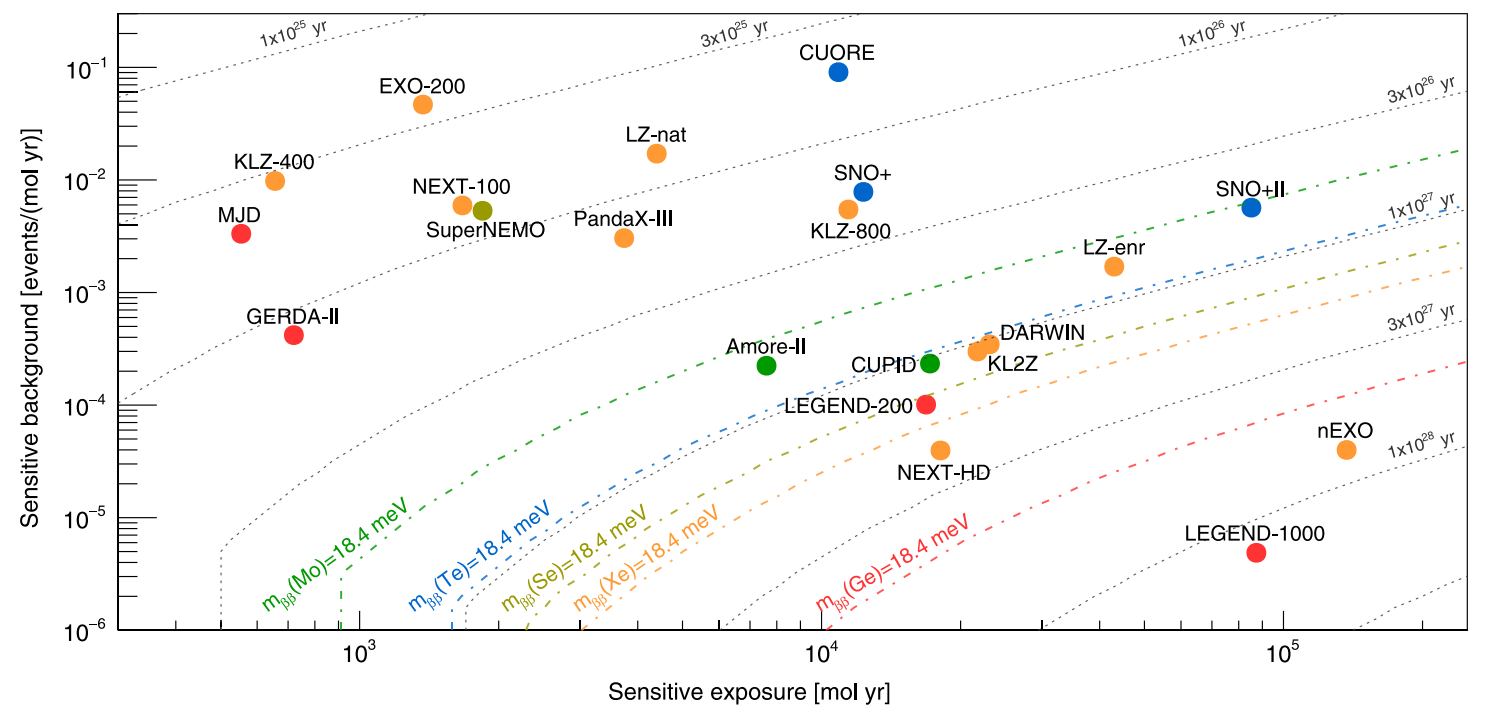
\includegraphics[width=\textwidth]{figures/experiments_and_sensitivities.png}
    \caption{Overview of the experiments searching for $0\nu\beta\beta$ decays with related sensitive exposures and backgrounds. Experiments marked in green exploit ${}^{100}$Mo, those in yellow use ${}^{136}$Xe, the blue ones employ ${}^{130}$Te, SuperNEMO is the only one using ${}^{82}$Se and finally red experiments exploit ${}^{76}$Ge. Plot taken from \cite{plot-esperiments_and_exposures}.}
    \label{fig:experiments-and-sensitivities-0nubb}
\end{figure}

% --- ACRONIMI E BIBLIOGRAFIA ---
\renewcommand{\chapterTitleSize}{\fontsize{36pt}{44pt}\selectfont}

\chapter*{List of Acronyms}
\addcontentsline{toc}{chapter}{List of Acronyms}

\begin{multicols}{2}
    \printacronyms[heading=none]
\end{multicols}

\cleardoublepage
\phantomsection
\addcontentsline{toc}{chapter}{Bibliography}
\printbibliography

\end{document}